% !TeX root = digital-platform-api-economy.tex
% !TeX encoding = UTF-8
\chapter{Desain Kontrak API dengan OpenAPI}
\label{ch:ch09}

% Kolom rata kiri untuk tabel bab ini: G selebar sisa tabel, H selebar yang ditentukan.
\newcolumntype{G}{>{\raggedright\arraybackslash}X}
\newcolumntype{H}[1]{>{\raggedright\arraybackslash}p{#1}}
% Tanda kutip tunggal dibaca sebagai teks, supaya tanda pagar pada $ref tidak dianggap komentar.
\lstdefinestyle{ch09yaml}{language=yaml, morestring=[b]', captionpos=b, xleftmargin=8pt, columns=fullflexible, keepspaces=true}

\section*{Tujuan Pembelajaran}
\begin{itemize}
  \item Menjelaskan pendekatan \textit{contract-first} dan manfaatnya bagi kerja sama dengan vendor dan mitra.
  \item Membaca dan meninjau kontrak OpenAPI dari sisi bisnis maupun teknis.
  \item Menyusun kontrak OpenAPI sederhana untuk satu API prioritas.
\end{itemize}

\section{Pendahuluan}

Vendor Medikara+ dan klinik mitra menafsirkan kata berhasil secara berbeda. Vendor menganggap permintaan yang diterima sudah
berarti janji terkonfirmasi, sedangkan petugas klinik menunggu kepastian slot. Pemisalan wawancara pada Bab 8 memperlihatkan gejalanya:
petugas menelepon rumah sakit karena tidak yakin slot sudah terkunci. Misalkan 10 persen dari 2.400 pemesanan per hari diikuti telepon 3 menit. Bebannya
300 jam per bulan, atau Rp216 juta per tahun pada tarif Rp60.000 per jam. Pertanyaan kemudian muncul: di mana arti berhasil
ditulis, siapa yang menyepakatinya, dan kapan?

Kontrak \textit{Application Programming Interface} (API) menjawab pertanyaan itu. Kontrak yang disepakati sebelum pembangunan
mengurangi salah pengertian dan menyediakan dasar pengujian bersama. Bab ini menulis kontrak untuk API-01 Jadwal dan Janji Temu,
sesuai keputusan portofolio Bab 8. Kontrak diperlakukan sebagai perjanjian, sehingga pemilik produk dan analis ikut memeriksa isinya
tanpa harus memprogram. Kode status dan kunci idempotensi diambil dari Bab 5, \textit{scope} dan hak atas objek dari Bab 6, serta
kosakata layanan kesehatan dari Bab 7. \textit{API gateway} dan masa transisi versi dibahas di Bab 10, sedangkan portal pengembang
di Bab 11. Angka tambahan yang diawali kata ``Misalkan'' adalah asumsi latihan. Kesimpulan untuk organisasi nyata harus diuji dengan
wawancara, dokumen, dan pengukuran yang berizin. Hasil bab ini menjadi bagian C3 dalam cetak biru transformasi digital.

Rujukan utama bab ini dipakai untuk membedakan konsep dan membangun alasan keputusan, bukan untuk menggantikan penilaian konteks
organisasi. Struktur kontrak mengikuti OpenAPI 3.2.0 \cite{openapi32}, dan aturan isian data mengikuti JSON Schema Draft 2020-12
\cite{c09-jsonschema-validation}. Bentuk pesan galat mengikuti \textit{Request for Comments} (RFC) 9457 \cite{rfc9457}. Kontrak
berbasis pesan mengikuti AsyncAPI 3.1.0 \cite{asyncapi31}. Pola desain diambil dari Zimmermann dkk. \cite{zimmermann2022patterns}.
Bukti tentang perubahan yang merusak diambil dari Xavier dkk. \cite{c09-xavier2017} dan Espinha dkk. \cite{espinha2014}.

\IfFileExists{../figures/ch09-diagram-konsep.png}{%

Gambar \ref{fig:ch09-ilustrasi-bab} merangkum hubungan komponen dan konsep utama bab ini.
\begin{figure}[!htb]
  \centering
  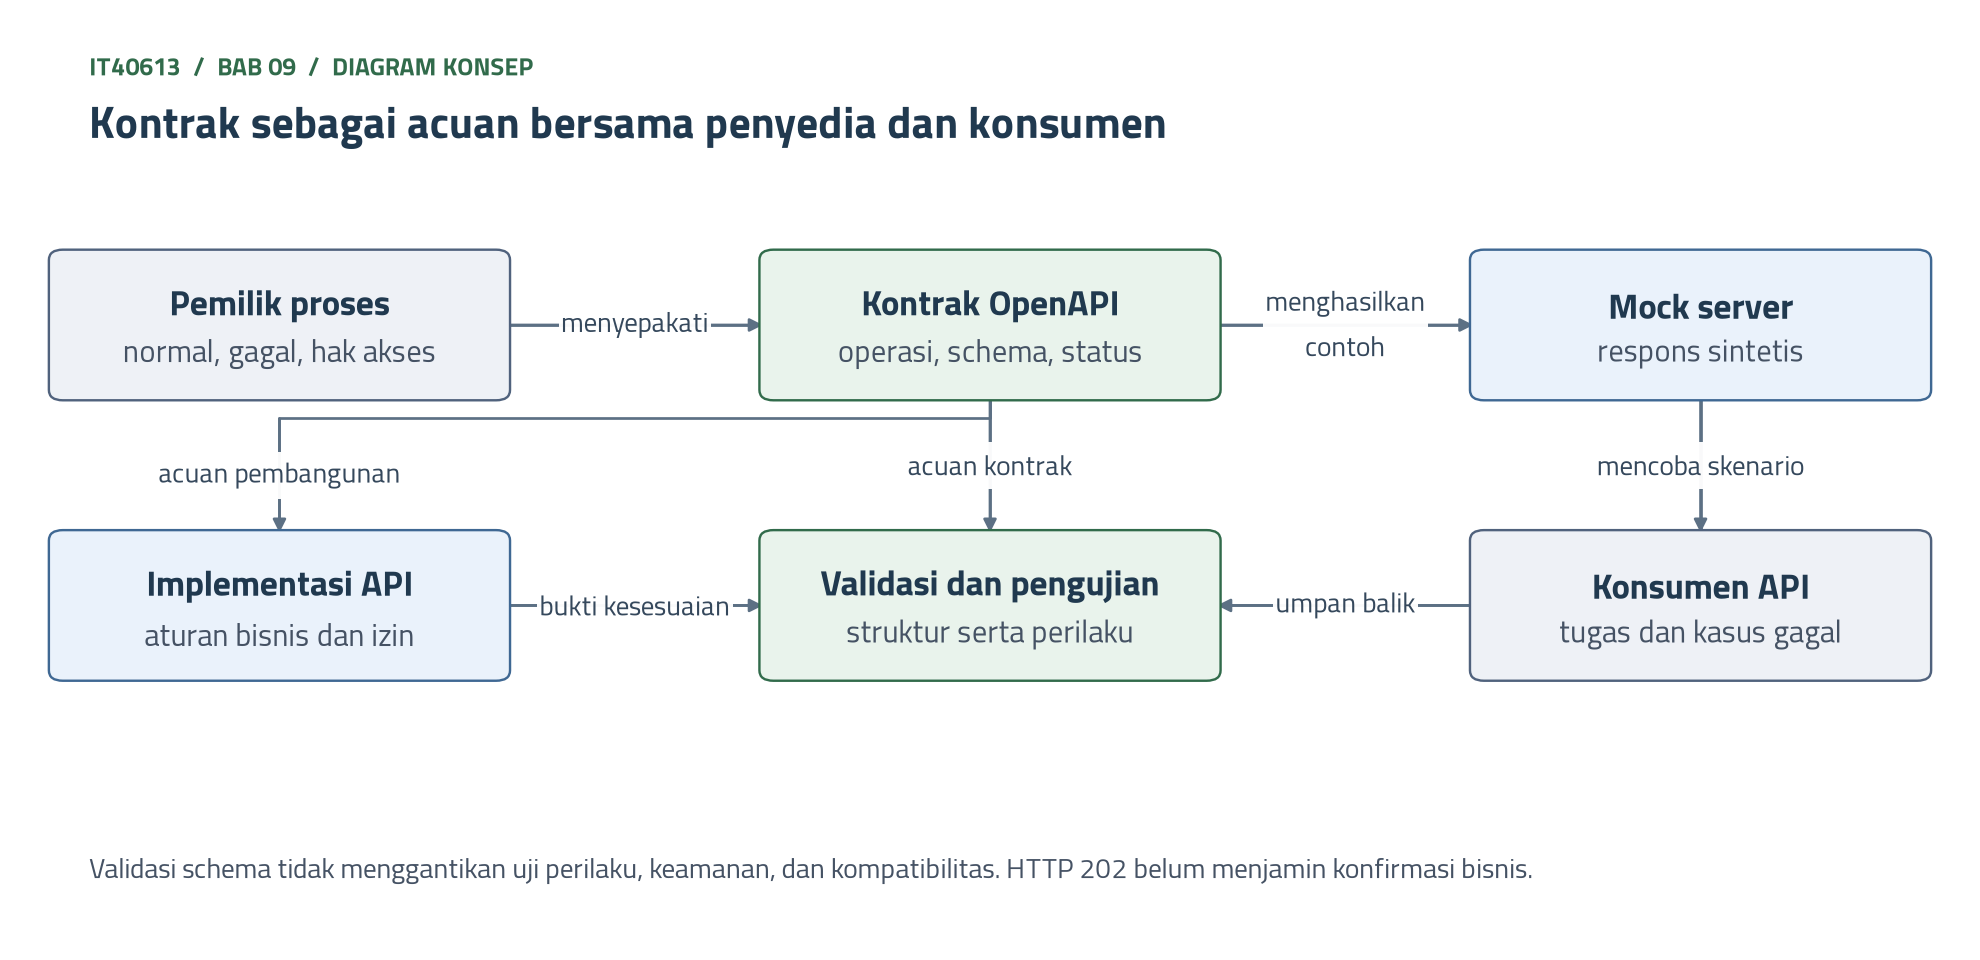
\includegraphics[width=\textwidth]{../figures/ch09-diagram-konsep.png}
  \caption{Kontrak sebagai acuan bersama penyedia dan konsumen}
  \label{fig:ch09-ilustrasi-bab}
\end{figure}
}{}

\section{Kontrak API dan Pendekatan Contract-First}

Vendor dan klinik sama-sama merasa benar, karena arti berhasil tidak pernah ditulis. Apa yang seharusnya ditulis, dan kapan?

Kontrak API adalah kesepakatan tertulis antara penyedia dan konsumen tentang perilaku antarmuka. Penyedia adalah pihak yang
menjalankan API, konsumen adalah pihak yang memakainya, dan klien adalah aplikasi milik konsumen. Kontrak memuat operasi, data,
autentikasi, respons, dan kondisi gagal. Spesifikasi OpenAPI merumuskan tujuan yang sama. OpenAPI mendefinisikan antarmuka standar
bagi API \textit{HyperText Transfer Protocol} (HTTP), sehingga manusia dan komputer dapat memahami kemampuan layanan tanpa membaca
kode sumber atau mengintip lalu lintas jaringan \cite{openapi32}. Zimmermann dkk. mencatat pola yang sama dengan nama API Description,
yang juga dikenal sebagai Explicit Service Contract \cite{zimmermann2022patterns}. Pendekatan \textit{contract-first} menyepakati
kontrak itu sebelum implementasi rinci. Bentuknya berkas teks berformat \textit{YAML Ain't Markup Language} (YAML) yang dapat dibaca
manusia. Kontrak teknis dibaca bersama aturan bisnis, seperti kapan slot dianggap terkunci di Sistem Informasi Manajemen Rumah Sakit
(SIMRS). Perubahan kontrak ditinjau penyedia serta konsumen, supaya keputusan tidak hanya mencerminkan kemudahan vendor.

Analoginya gambar kerja rumah. Gambar kerja disepakati sebelum pembangunan, sehingga pembeli dan pelaksana mempunyai rujukan yang
sama. Pembeli yang tidak mengerti teknik sipil tetap dapat membaca letak pintu dan jumlah kamar. Memindahkan pintu pada gambar hanya
menghapus garis, sedangkan memindahkan pintu sesudah tembok berdiri berarti membongkar.

Dua contoh berangka pada Medikara:
\begin{enumerate}
  \item Misalkan 202 berarti permintaan masuk antrean, sedangkan 201 berarti janji dibuat. Perbedaan ini menentukan pesan yang
        ditampilkan kepada pasien. RFC 9110 menyatakan kode 202 hanya berarti permintaan diterima untuk diproses, dan permintaan itu
        masih mungkin tidak dijalankan \cite{rfc9110}. Misalkan aplikasi menampilkan 202 sebagai berhasil, lalu 2 persen antrean
        berakhir dengan slot penuh. Dari 2.400 pemesanan per hari, ada 48 pasien yang datang tanpa janji, atau 1.200 per bulan pada
        25 hari kerja. Dengan 10 menit penanganan di loket, bebannya 200 jam per bulan, atau Rp144 juta per tahun.
  \item Misalkan arti terkonfirmasi dibahas pada tinjauan kontrak oleh 5 orang selama 2 jam, atau 10 jam dan Rp600.000. Bila salah
        pengertian itu baru ditemukan sesudah vendor membangun, vendor memerlukan 80 jam perbaikan. Bab 4 memisalkan satu perubahan
        menyita 4 jam per klinik, atau 160 jam untuk 40 klinik. Jumlahnya 240 jam, atau Rp14,4 juta. Temuan yang sama menjadi 24 kali
        lebih mahal hanya karena waktunya berbeda.
\end{enumerate}

Gambar \ref{fig:ch09-alur} menempatkan kedua hitungan itu pada garis waktu. Vendor Medikara+ menyatakan butuh 4 bulan untuk mengubah
aplikasi, seperti pada pemisalan Bab 8. Pada lajur atas, klinik sudah dapat mencoba pada minggu ketiga. Pada lajur bawah, klinik baru
mencoba pada bulan kelima.

\begin{figure}[!htb]
  \centering
  \begin{tikzpicture}[
  font=\scriptsize,
  execute at begin node={\hyphenpenalty=10000\exhyphenpenalty=10000},
  lajur/.style={draw, rounded corners, fill=praditagreen!15, text width=1.75cm, minimum height=1.45cm, align=center},
  tahap/.style={draw, rounded corners, fill=blue!8, text width=1.65cm, minimum height=1.45cm, align=center},
  tekan/.style={tahap, fill=orange!12},
  hasil/.style={tahap, fill=green!10},
  masalah/.style={tahap, fill=red!22},
  panah/.style={-{Stealth[length=2mm]}, thick}
]
  % Lajur atas menaruh temuan di awal, lajur bawah menaruh temuan sesudah pembangunan.
  \node[lajur] (a0) at (-0.1,0) {\textbf{Contract-first}};
  \node[tahap] (a1) at (2.15,0) {Aturan bisnis ditulis\\{\tiny\mdseries minggu 1}};
  \node[tekan] (a2) at (4.3,0) {Kontrak disepakati\\{\tiny\mdseries minggu 2}};
  \node[tahap] (a3) at (6.45,0) {5 klinik mencoba mock\\{\tiny\mdseries minggu 3}};
  \node[tahap] (a4) at (8.6,0) {Vendor membangun\\{\tiny\mdseries bulan 1 sampai 4}};
  \node[hasil] (a5) at (10.75,0) {Implementasi diuji terhadap kontrak};
  \draw[panah] (a1) -- (a2);
  \draw[panah] (a2) -- (a3);
  \draw[panah] (a3) -- (a4);
  \draw[panah] (a4) -- (a5);

  \node[lajur] (b0) at (-0.1,-2.35) {\textbf{Code-first}};
  \node[tahap] (b1) at (2.15,-2.35) {Vendor membangun menurut tafsirnya\\{\tiny\mdseries bulan 1 sampai 4}};
  \node[tahap] (b2) at (4.3,-2.35) {Dokumentasi ditulis dari kode};
  \node[tahap] (b3) at (6.45,-2.35) {Klinik mencoba\\{\tiny\mdseries bulan 5}};
  \node[masalah] (b4) at (8.6,-2.35) {Salah arti ditemukan};
  \node[tahap] (b5) at (10.75,-2.35) {Perbaikan vendor dan 40 klinik};
  \draw[panah] (b1) -- (b2);
  \draw[panah] (b2) -- (b3);
  \draw[panah] (b3) -- (b4);
  \draw[panah] (b4) -- (b5);

  \node[anchor=north, text width=3.6cm, align=center] at (4.3,-0.8) {{\tiny\mdseries Temuan di sini: 10 jam, Rp600.000}};
  \node[anchor=north, text width=3.6cm, align=center] at (9.7,-3.15) {{\tiny\mdseries Temuan di sini: 240 jam, Rp14,4 juta}};
\end{tikzpicture}

  \caption{Pendekatan \textit{contract-first} memindahkan temuan salah arti ke awal pekerjaan}
  \label{fig:ch09-alur}
\end{figure}

Siapa yang membaca kontrak, dan bagian mana yang ia periksa? Kontrak bukan hanya urusan pemrogram. Tabel \ref{tab:ch09-baca-kontrak}
memperlihatkan pertanyaan yang dijawab kontrak bagi pemilik produk dan analis. Tiap bagian dijelaskan lagi pada seksi Struktur OpenAPI
3.2. Pada API-01, pemilik proses sekaligus pemilik produk, yaitu Manajer Layanan Rawat Jalan.

\begin{table}[!htb]
  \centering
  \caption{Kontrak sebagai perjanjian: pertanyaan pembaca, bagian yang dibaca, dan pemberi isi pada API-01}
  \label{tab:ch09-baca-kontrak}
  \footnotesize
  \begin{tabularx}{\textwidth}{GH{2.1cm}GH{2.5cm}}
    \hline
    \textbf{Pertanyaan pembaca} & \textbf{Bagian kontrak} & \textbf{Jawaban pada API-01} & \textbf{Pemberi isi} \\ \hline
    Kemampuan apa yang dibuka dan siapa penanggung jawabnya? & \texttt{info} & Jadwal dan janji temu, Manajer Layanan Rawat Jalan & Pemilik proses \\ \hline
    Apa yang boleh dilakukan konsumen? & \texttt{paths} & Cari jadwal, buat janji, baca status, batalkan & Pemilik proses, analis \\ \hline
    Data apa yang masuk dan keluar? & \textit{schema} & Slot dan nomor pasien, tanpa isi rekam medis & Petugas pelindungan data \\ \hline
    Apa arti berhasil? & \texttt{responses} 2xx & 201 terkonfirmasi, 202 menunggu & Pemilik proses \\ \hline
    Apa arti gagal dan apa langkah berikutnya? & \texttt{responses} 4xx, 5xx & 409 slot terisi, aplikasi menawarkan slot lain & Layanan pelanggan \\ \hline
    Siapa yang boleh memanggil? & \texttt{security} & Klinik dengan \textit{scope} \texttt{janji.tulis} & Keamanan \\ \hline
  \end{tabularx}
\end{table}

Dua hal pada kontrak sering tertukar, yaitu kontrak API dan perjanjian kerja sama. Pembagiannya begini. Kontrak API mengatur perilaku
antarmuka: operasi, data, dan arti jawaban. Perjanjian kerja sama mengatur hubungan hukum: harga, tanggung jawab, kerahasiaan, dan
penyelesaian sengketa. Janji mutu layanan yang terukur, misalnya ketersediaan, punya pola sendiri, yaitu Service Level Agreement
\cite{zimmermann2022patterns}. Langganan Rp3 juta per klinik per bulan pada skema Bab 2 tertulis di perjanjian kerja sama, sedangkan
409 tertulis di kontrak API. Kuota 300 panggilan per hari per klinik muncul di keduanya, sehingga angkanya wajib sama.

Apakah kontrak selalu harus ditulis lebih dulu? Tidak selalu. Tabel \ref{tab:ch09-contract-first} membandingkan \textit{contract-first}
dengan \textit{code-first}, yaitu menulis kode lebih dulu lalu menurunkan dokumentasi darinya.

\begin{table}[!htb]
  \centering
  \caption{\textit{Contract-first} dan \textit{code-first} beserta \textit{tradeoff}-nya}
  \label{tab:ch09-contract-first}
  \footnotesize
  \begin{tabularx}{\textwidth}{H{2.8cm}GG}
    \hline
    \textbf{Unsur} & \textbf{\textit{Contract-first}} & \textbf{\textit{Code-first}} \\ \hline
    Kesepakatan & Sebelum pembangunan & Sesudah kode berjalan \\ \hline
    Peserta & Pemilik proses, vendor, konsumen & Terutama tim pembangun \\ \hline
    Kerja bersama & Konsumen mencoba \textit{mock server} lebih awal & Konsumen menunggu API berjalan \\ \hline
    Risiko utama & Waktu rapat di awal, kontrak dapat basi bila tidak dijaga & Salah arti ditemukan terlambat, bentuk API mengikuti struktur internal \\ \hline
    Cocok untuk & Banyak konsumen, vendor terpisah, data sensitif & API internal satu tim, percobaan yang umurnya pendek \\ \hline
    Pada Medikara & API-01: 40 klinik, 1 vendor, 5 SIMRS & Misalkan alat internal tim integrasi \\ \hline
  \end{tabularx}
\end{table}

Keputusan memakai \textit{contract-first} punya dua konsekuensi. Pertama, ada biaya sebelum kode pertama ditulis. Misalkan tiga sesi
2 jam diikuti 5 orang. Biayanya 30 jam, atau Rp1,8 juta. Angka itu kecil dibanding Rp14,4 juta untuk satu temuan yang terlambat, tetapi
waktu pemilik proses harus benar-benar tersedia. Kedua, kontrak harus dijaga tetap sama dengan implementasi. Kontrak yang basi lebih
berbahaya daripada tidak ada kontrak, karena konsumen memercayainya. Diagram konsep bab ini memperlihatkan kewajiban itu: implementasi
menyerahkan bukti kesesuaian kepada validasi dan pengujian, dan umpan balik konsumen masuk ke tempat yang sama.

Seberapa luas pendekatan ini dipakai? Laporan Postman mencatat 82 persen organisasi mengadopsi \textit{API-first} pada tingkat tertentu,
dan 25 persen menyebut diri sepenuhnya \textit{API-first} \cite{postman2025}. Angka itu perlu dibaca hati-hati karena dua alasan. Postman
menjual alat API, dan angka tersebut adalah pengakuan responden, bukan pengukuran manfaat. \textit{API-first} juga lebih luas daripada
\textit{contract-first}, karena memperlakukan API sebagai produk. Yang dapat diambil lebih sempit: praktik ini umum, sehingga vendor
dapat diminta menjalankannya, tetapi manfaatnya bagi Medikara tetap harus diukur dari telepon konfirmasi.

\begin{kasus}[title={Kasus Medikara Health: Arti Berhasil pada API-01}]
Misalkan Manajer Layanan Rawat Jalan, tim integrasi, vendor Medikara+, dan wakil 5 klinik bertemu dua jam, sebelum vendor menulis kode.
Seluruh rincian ini adalah data latihan. Rapat dimulai dari satu kalimat petugas klinik: ``Saat layar menulis berhasil, apakah pasien
boleh pulang?'' Vendor menjawab belum tentu, karena beberapa SIMRS memproses permintaan sesudah beberapa detik.

Rapat menghasilkan tiga keputusan.
\begin{enumerate}
  \item Hanya 201 yang berarti slot sudah terkunci di SIMRS. Layar menulis ``janji terkonfirmasi''.
  \item Kode 202 berarti permintaan masih diproses. Layar menulis ``menunggu kepastian'', dan aplikasi membaca status sampai jawabannya
        pasti. Misalkan 5 persen pemesanan berakhir di 202, atau 120 per hari. Bila satu janji rata-rata dibaca 5 kali, ada 600 panggilan
        per hari, atau 15 per klinik. Kebutuhan satu klinik naik dari 180 menjadi 195 panggilan, masih di bawah kuota 300.
  \item Kode 409 berarti slot terisi dan janji tidak dibuat. Aplikasi menawarkan slot lain tanpa mengantre ulang.
\end{enumerate}

Sebuah usulan belum menjadi keputusan sebelum pemilik menerima konsekuensinya. Manajer Layanan Rawat Jalan menerima bahwa sebagian
pasien harus menunggu beberapa detik sebelum mendapat kepastian. Sebagai gantinya, telepon konfirmasi ditargetkan turun dari 10 ke 2
persen seperti pada kanvas Bab 8, atau dari 240 menjadi 48 telepon per hari. Bila tercapai, beban turun dari 300 menjadi 60 jam per bulan,
sehingga terhemat Rp172,8 juta per tahun. Angka itu masih target, dan bukti yang dapat mengubah keputusan adalah catatan telepon nyata.
\end{kasus}

\section{Pemodelan Sumber Daya dan Penamaan}

Arti berhasil sudah ditulis. Berikutnya, kontrak membutuhkan kata benda: hal apa yang dibicarakan penyedia dan konsumen?

Sumber daya merepresentasikan hal yang dikenali pengguna, misalnya jadwal dan janji temu. Nama yang stabil serta pengenal yang tidak
membocorkan struktur internal memudahkan pemakaian. Metode HTTP dan perubahan status menjelaskan tindakan atas sumber daya itu. Informasi
yang diperlukan untuk memutuskan tindakan tidak boleh disembunyikan dalam asumsi pengembang. Kontrak yang baik dapat dibaca petugas klinik
sebagai daftar hal yang ia kenal, bukan sebagai daftar tabel.

Analoginya nomor antrean. Nomor antrean tetap dikenali meskipun petugas loket berganti atau komputer loket diperbarui. Pasien tidak perlu
tahu nomor itu disimpan di buku mana. Nomor antrean juga tidak membuktikan hak: memegang nomor orang lain tidak membuat seseorang berhak
atas layanan orang itu.

Dua contoh berangka pada Medikara:
\begin{enumerate}
  \item \texttt{GET /jadwal-dokter} dari Bab 1 mengembalikan slot beserta pengenalnya. \texttt{POST /janji-temu} memakai pengenal itu dan
        tetap memeriksa apakah slot masih tersedia. Pemeriksaan kedua wajib ada, karena Bab 5 membolehkan jawaban jadwal disimpan di
        \textit{cache} lima menit, sehingga daftar slot dapat basi. Bab 5 memisalkan 280 pemesanan per bulan bentrok, atau 1 persen dari
        28.000. Kontrak menjawab semuanya dengan 409, bukan dengan janji ganda.
  \item Pengenal janji \texttt{JT-40771} stabil dan dipakai untuk pembatalan serta rekonsiliasi, walaupun lima SIMRS memakai penomoran
        sendiri. Nomor urut basis data tidak diperlakukan sebagai bukti kewenangan. Misalkan pengenal berurutan dan layanan hanya memeriksa
        token. Dengan kuota 300 per hari, satu klinik dapat mencoba 9.000 nomor dalam 30 hari. Risiko ini tercatat sebagai kelemahan
        otorisasi tingkat objek pada \textit{Open Worldwide Application Security Project} (OWASP) \cite{owasp-api1}, seperti pada Bab 6.
\end{enumerate}

Kata apa yang dipakai dalam kontrak? Bab 8 mencatat kunjungan, janji temu, dan Encounter sering tertukar, sehingga kosakata disepakati
sebelum kontrak ditulis. Tabel \ref{tab:ch09-kosakata} memuat hasilnya. Pada \textit{Health Level Seven Fast Healthcare Interoperability Resources}
(HL7 FHIR) R4, Appointment adalah pemesanan untuk waktu tertentu yang
dapat menghasilkan satu atau lebih Encounter \cite{c09-fhir-appointment}, sedangkan Slot adalah rentang waktu pada jadwal yang dapat dipesan
\cite{c09-fhir-slot}. Pembagian itu sejajar dengan kebutuhan API-01, walaupun API-01 tidak memakai format FHIR.

\begin{table}[!htb]
  \centering
  \caption{Kosakata kontrak API-01, satu kata untuk satu arti}
  \label{tab:ch09-kosakata}
  \footnotesize
  \begin{tabularx}{\textwidth}{H{2.2cm}GH{2.8cm}H{1.8cm}}
    \hline
    \textbf{Kata} & \textbf{Arti dalam kontrak} & \textbf{Bukan berarti} & \textbf{Padanan FHIR} \\ \hline
    Slot & Satu rentang waktu yang dapat dipesan & Janji temu & Slot \\ \hline
    Janji temu & Pemesanan seorang pasien atas satu slot & Kunjungan & Appointment \\ \hline
    Kunjungan & Pertemuan layanan yang benar-benar terjadi, di luar API-01 & Janji temu & Encounter \\ \hline
    Terkonfirmasi & Slot sudah terkunci di SIMRS & Permintaan sudah diterima & Tidak dipetakan \\ \hline
    Menunggu & Permintaan diterima, hasilnya belum pasti & Janji pasti ada & Tidak dipetakan \\ \hline
  \end{tabularx}
\end{table}

Bagaimana nama ditulis? Kontrak API-01 memakai empat kebiasaan. Nama sumber daya berupa kata benda dengan huruf kecil dan tanda hubung,
seperti \texttt{/janji-temu}. Nama bidang mengikuti contoh Bab 5, seperti \texttt{rumahSakit}. Nama tidak boleh meniru nama tabel. Nilai
pengenal tidak boleh mengandung nama sistem atau vendor, sehingga pergantian vendor tidak mengubah kontrak.

Kanvas Bab 8 menyebut lima kata kerja: cari jadwal, pilih slot, kunci slot, batalkan, dan baca status. Apakah kontrak memerlukan lima
operasi? Tidak. Memilih slot terjadi di layar konsumen, sehingga tidak ada yang perlu dijawab server. Mengunci slot adalah bagian dari
membuat janji, supaya tidak ada slot yang terkunci tanpa pasien. Hasilnya empat operasi. Gambar \ref{fig:ch09-status} memperlihatkan perubahan
status akibat operasi itu.

\begin{figure}[!htb]
  \centering
  \begin{tikzpicture}[
  font=\scriptsize,
  execute at begin node={\hyphenpenalty=10000\exhyphenpenalty=10000},
  kotak/.style={draw, rounded corners, fill=blue!8, text width=2.3cm, minimum height=1.0cm, align=center},
  tekan/.style={kotak, fill=orange!12},
  hasil/.style={kotak, fill=green!10},
  masalah/.style={kotak, fill=red!22},
  redup/.style={kotak, fill=gray!35},
  label/.style={font=\tiny, fill=white, inner sep=1pt, align=center},
  panah/.style={-{Stealth[length=2mm]}, thick}
]
  % Hanya status terkonfirmasi yang boleh dibaca sebagai janji pasti.
  \node[kotak] (minta) at (0,0) {\texttt{POST /janji-temu}\\{\tiny\mdseries slot dan pasien}};
  \node[hasil] (konfirm) at (4.7,1.55) {\textbf{terkonfirmasi}\\{\tiny\mdseries slot sudah terkunci}};
  \node[tekan] (tunggu) at (4.7,0) {\textbf{menunggu}\\{\tiny\mdseries hasil belum pasti}};
  \node[masalah] (tanpa) at (4.7,-1.55) {Tanpa janji\\{\tiny\mdseries pilih slot lain}};
  \node[redup] (batal) at (9.4,1.55) {\textbf{dibatalkan}\\{\tiny\mdseries data tetap disimpan}};
  \node[masalah] (tolak) at (9.4,0) {\textbf{ditolak}\\{\tiny\mdseries slot terisi saat diproses}};
  \node[draw, dashed, rounded corners, text width=2.3cm, minimum height=0.8cm, align=center] (kunjungan) at (9.4,3.0)
    {Kunjungan\\{\tiny\mdseries Encounter, di luar API-01}};

  \draw[panah] (minta.north) |- node[label, pos=0.75] {201} (konfirm.west);
  \draw[panah] (minta) -- node[label] {202} (tunggu);
  \draw[panah] (minta.south) |- node[label, pos=0.75] {409} (tanpa.west);
  \draw[panah] (tunggu) -- node[label] {slot terkunci} (konfirm);
  \draw[panah] (tunggu) -- node[label] {slot terisi} (tolak);
  \draw[panah] (konfirm) -- node[label] {\texttt{DELETE}, 200} (batal);
  \draw[panah] (tunggu.north east) -- node[label, pos=0.45] {\texttt{DELETE}, 200} (batal.south west);
  \draw[panah, dashed] (konfirm.north) |- node[label, pos=0.75] {pasien datang} (kunjungan.west);
\end{tikzpicture}

  \caption{Status janji temu pada API-01. Hanya status terkonfirmasi yang berarti janji pasti}
  \label{fig:ch09-status}
\end{figure}

Menyatakan status secara tertulis punya dua konsekuensi. Pertama, \texttt{GET /janji-temu/\{id\}} menjadi operasi wajib, sesuai temuan
wawancara 5 klinik pada Bab 8. Kedua, batas API-01 menjadi jelas. Kehadiran pasien adalah kunjungan, sehingga status ``hadir'' atau ``selesai''
tidak ditambahkan di sini. Bila ditambahkan, API-01 ikut memegang aturan yang pemiliknya berbeda.

Aturan bisnis apa yang masih tersembunyi? Tim menulisnya dalam bahasa biasa pada \berkas{sources/chapter09/lembar-aturan-bisnis.md}. Misalkan
pembatalan paling lambat dua jam sebelum slot mulai, karena dokter sudah bersiap. Aturan itu tidak terlihat pada bentuk data, tetapi konsumen
perlu mengetahuinya. Karena itu kontrak menuliskannya pada ringkasan operasi dan menjawabnya dengan 409.

\subsection{Pola Desain API}

Banyak keputusan pada API-01 sudah pernah dihadapi organisasi lain. Apakah tim harus memikirkannya dari nol?

Pola desain adalah solusi yang sudah diuji untuk masalah yang berulang. Zimmermann dkk. menulis katalog pola API, dan tiap pola menjawab satu
pertanyaan desain, misalnya bagaimana mengirim data yang besar tanpa membebani klien \cite{zimmermann2022patterns}. Pola bukan aturan wajib.
Pola memberi nama bersama dan akibat yang sudah dikenal, sehingga rapat dapat membahas pilihan dengan lebih cepat.

Analoginya pola jahit. Penjahit tidak menggambar kemeja dari nol. Pola menentukan potongan dasar, lalu ukurannya disesuaikan dengan pemesan.
Pola yang cocok untuk seragam belum tentu cocok untuk kebaya.

Dua contoh berangka pada Medikara:
\begin{enumerate}
  \item Pola Rate Limit menjawab cara mencegah pemakaian berlebihan. Bab 3 menetapkan kuota 300 panggilan per hari per klinik dari kebutuhan
        180 panggilan. Cadangannya 120 panggilan per klinik. Untuk 40 klinik, kebutuhan 7.200 panggilan per hari setara 60 persen dari
        kapasitas 12.000.
  \item Misalkan vendor mengusulkan pola Request Bundle, supaya 60 pemesanan harian satu klinik dikirim sekaligus. Panggilan turun dari 60
        menjadi 1. Namun pemesanan terjadi satu per satu saat pasien menunggu, dan 1 persen yang bentrok membuat jawaban harus membawa hasil per
        butir. Cadangan kuota masih 120 panggilan, sehingga masalah yang hendak diselesaikan belum ada. Pola ditolak secara tertulis.
\end{enumerate}

Tabel \ref{tab:ch09-pola} memuat pola yang dipakai API-01. Nama pola sengaja tidak diterjemahkan, supaya mudah dicari pada katalognya.
Visibilitas API mengikuti Bab 8. Bagi klinik mitra, API-01 adalah Community API, karena aksesnya terbatas pada kelompok badan hukum tertentu.

\begin{table}[!htb]
  \centering
  \caption{Pola desain API dari katalog Zimmermann dkk. dan penerapannya pada API-01}
  \label{tab:ch09-pola}
  \footnotesize
  \begin{tabularx}{\textwidth}{H{2.8cm}GG}
    \hline
    \textbf{Pola} & \textbf{Pertanyaan yang dijawab} & \textbf{Penerapan pada API-01} \\ \hline
    Retrieval Operation & Bagaimana mengambil informasi dari penyedia? & \texttt{GET /jadwal-dokter} \\ \hline
    State Creation Operation & Bagaimana klien melaporkan hal yang perlu diproses penyedia? & \texttt{POST /janji-temu} \\ \hline
    State Transition Operation & Bagaimana klien memicu perubahan keadaan di penyedia? & \texttt{DELETE /janji-temu/\{id\}} mengubah status \\ \hline
    Operational Data Holder & Bagaimana melayani data berumur pendek yang sering berubah? & Janji temu \\ \hline
    Id Element & Bagaimana membedakan elemen API satu sama lain? & \texttt{JT-40771}, \texttt{BKS-20261102-0915} \\ \hline
    Pagination & Bagaimana mengirim banyak data tanpa membebani klien? & Parameter \texttt{batas} dan \texttt{kursor} \\ \hline
    Error Report & Bagaimana memberi tahu kesalahan kepada klien? & \textit{Problem Details} \\ \hline
    Rate Limit & Bagaimana mencegah pemakaian berlebihan? & 300 panggilan per hari per klinik, kode 429 \\ \hline
    Version Identifier & Bagaimana menyatakan kemampuan dan perubahan yang tidak cocok? & \texttt{info.version} \\ \hline
  \end{tabularx}
\end{table}

\section{Model Galat, Pagination, dan Penyaringan}

Kontrak yang lemah biasanya rapi pada jalur berhasil dan kosong pada jalur gagal. Padahal petugas klinik paling membutuhkan kontrak saat ada
yang salah. Bab 5 sudah menunjukkan akibatnya: API yang menjawab 200 dan menaruh kata ``gagal'' di isi jawaban menyembunyikan 280 bentrok per
bulan. Apa yang perlu dijanjikan saat gagal?

\textit{Problem Details} dalam RFC 9457 menyediakan bentuk terstruktur untuk galat (\textit{error}) HTTP. RFC ini menggantikan RFC 7807. Pesan
galat berupa objek \textit{JavaScript Object Notation} (JSON) dengan jenis media \berkas{application/problem+json} dan lima bidang: \texttt{type},
\texttt{status}, \texttt{title}, \texttt{detail}, dan \texttt{instance}. Bidang \texttt{type} adalah pengenal utama jenis masalah, sehingga konsumen
memutuskan tindakan dari bidang itu, bukan dari kalimat. Bidang \texttt{title} adalah ringkasan singkat yang sama untuk satu jenis masalah.
Bidang \texttt{detail} menjelaskan kejadian yang satu ini. Bidang \texttt{instance} menandai kejadian tertentu, yang berguna bagi dukungan dan
penelusuran \cite{rfc9457}. Tipe masalah membantu klien menentukan penanganan, tetapi detail tidak boleh membocorkan rahasia.

Analoginya surat penolakan. Surat yang baik menjelaskan jenis masalah dan cara memperbaikinya tanpa membuka arsip internal petugas. Nomor surat
memudahkan pemohon menanyakan kasusnya. Pemohon tidak perlu tahu nama pegawai yang memeriksa atau isi map di meja.

Dua contoh berangka pada Medikara:
\begin{enumerate}
  \item Konflik slot memakai status 409 dengan tipe masalah slot terisi. RFC 9110 mengartikan 409 sebagai konflik dengan keadaan sumber daya yang
        masih mungkin diselesaikan pengguna \cite{rfc9110}. Klien kemudian menawarkan jadwal lain. Misalkan tanpa tipe yang jelas, 280 bentrok per
        bulan masing-masing berakhir dengan telepon 6 menit. Bebannya 28 jam per bulan, atau Rp20,16 juta per tahun.
  \item Bab 5 mencatat jadwal kosong 7 sampai 14 hari per tahun saat SIMRS diperbarui. Bila API menjawab 200 dengan daftar kosong, petugas mengira
        dokter tidak praktik. Pada 2.400 pemesanan per hari, ada 16.800 sampai 33.600 pemesanan per tahun yang mendapat jawaban keliru. Kontrak
        membedakan keduanya: 200 dengan daftar kosong berarti tidak ada slot, sedangkan 503 berarti SIMRS sedang diperbarui, disertai
        \textit{header} \texttt{Retry-After}. Ini sekaligus rencana cadangan yang diwajibkan Bab 8 bagi API-01.
\end{enumerate}

Tabel \ref{tab:ch09-galat} memuat seluruh galat API-01. Kolom terakhir tidak dikirim kepada konsumen. Enam skenario gagal pada Bab 3 terwakili di
sini, kecuali penjamin menolak. Verifikasi penjaminan adalah kandidat lanjutan pada Bab 8, sehingga skenario itu dicatat di luar API-01, dan
skenario SIMRS diperbarui ditambahkan sebagai gantinya.

\begin{table}[!htb]
  \centering
  \caption{Model galat API-01: kode, tipe masalah, tindakan, dan catatan internal}
  \label{tab:ch09-galat}
  \scriptsize
  \begin{tabularx}{\textwidth}{H{0.6cm}H{2.8cm}GGG}
    \hline
    \textbf{Kode} & \textbf{Tipe masalah} & \textbf{Pesan bagi petugas} & \textbf{Tindakan konsumen} & \textbf{Hanya di catatan internal} \\ \hline
    400 & \berkas{masukan-tidak-sah} & Periksa tanggal dan bidang isian & Perbaiki isian & Nilai yang ditolak \\ \hline
    400 & \berkas{pasien-tidak-dapat-dipakai} & Nomor pasien tidak dapat dipakai. Periksa kartu pasien & Periksa nomor, jangan menebak & Apakah pasien ada \\ \hline
    401 & \berkas{token-tidak-sah} & Akses kedaluwarsa & Minta token baru & Alasan token ditolak \\ \hline
    403 & \berkas{akses-tidak-cukup} & Klinik belum punya hak ini & Hubungi pemilik kemitraan & \textit{Scope} yang kurang \\ \hline
    404 & \berkas{janji-tidak-ditemukan} & Janji tidak ditemukan & Periksa nomor janji & Klinik pemilik janji \\ \hline
    409 & \berkas{slot-terisi} & Slot sudah terisi. Pilih slot lain & Tawarkan slot lain & Pemegang slot \\ \hline
    409 & \berkas{pembatalan-terlambat} & Slot mulai kurang dari dua jam lagi. Hubungi rumah sakit & Tampilkan nomor rumah sakit & Waktu permintaan \\ \hline
    429 & \berkas{kuota-habis} & Kuota hari ini habis & Tunda sesuai \texttt{Retry-After} & Jumlah panggilan \\ \hline
    503 & \berkas{simrs-tidak-tersedia} & Jadwal belum dapat dibaca. Bukan berarti tidak ada dokter & Coba lagi sesuai \texttt{Retry-After} & SIMRS dan versinya \\ \hline
  \end{tabularx}
\end{table}

Dua hal pada pesan galat sering tertukar, yaitu pesan bagi mesin dan pesan bagi manusia. Pembagiannya begini. Bagi mesin, \texttt{type} dan kode
status menentukan langkah berikutnya. Bagi manusia, \texttt{title} dan \texttt{detail} menjelaskan keadaan. RFC 9457 meminta konsumen tidak mengurai
kalimat pada \texttt{detail} \cite{rfc9457}, karena satu perbaikan ejaan dapat merusak klinik. Karena itu kalimat boleh diperbaiki, sedangkan \texttt{type} diperlakukan sebagai janji.

Apa yang tidak boleh ada di pesan galat? RFC 9457 mengingatkan risiko bocornya informasi yang dapat dipakai menyerang sistem atau melanggar privasi
pengguna, termasuk rincian seperti \textit{stack dump} \cite{rfc9457}. Tiga keputusan API-01 mengikuti peringatan itu.
\begin{enumerate}
  \item Nomor pasien yang tidak dikenal dan nomor pasien yang bukan hak klinik itu dijawab sama, yaitu \berkas{pasien-tidak-dapat-dipakai}. Bila
        jawabannya berbeda, klinik dapat menebak nomor untuk mengetahui siapa yang menjadi pasien Medikara.
  \item Janji milik klinik lain dijawab 404, bukan 403. RFC 9110 membolehkan 404 bagi server yang ingin menyembunyikan keberadaan sumber daya
        terlarang \cite{rfc9110}. Bab 6 memakai 403 pada contoh hasil pemeriksaan. Keduanya sah. Kode 403 memudahkan pemanggil memahami sebabnya, sedangkan
        404 tidak mengungkapkan keberadaan objek. Pada kedua pilihan, percobaan itu tetap dicatat di sisi penyedia.
  \item Petugas dukungan memakai \texttt{instance}, misalnya \berkas{/kejadian/MSL-20261102-00731}. Petugas klinik cukup menyebut nomor itu, tanpa
        menyebut nama pasien lewat telepon.
\end{enumerate}

\begin{pendalaman}[title={Pendalaman Teknis (opsional): Membaca Contoh Problem Details}]
Listing \ref{lst:ch09-masalah} adalah contoh yang tertulis di kontrak. Kontrak ditulis dalam YAML, sedangkan
jawaban dikirim sebagai JSON dengan isi yang sama. RFC 9457 menganjurkan alamat \texttt{type} yang dapat dibuka, sehingga pengembang dapat membaca
penjelasan jenis masalah \cite{rfc9457}. Domain \texttt{.example} dicadangkan untuk contoh.

\begin{lstlisting}[style=ch09yaml, caption={Contoh galat slot terisi, tersedia di \berkas{sources/chapter09/kontrak-api-01-janji-temu.yaml}}, label={lst:ch09-masalah}]
    SlotTerisi:
      summary: Slot sudah dipakai pasien lain.
      value:
        type: https://api.medikara.example/masalah/slot-terisi
        title: Slot sudah terisi
        status: 409
        detail: Slot BKS-20261102-0915 sudah terisi. Pilih slot lain.
        instance: /kejadian/MSL-20261102-00731
\end{lstlisting}
\end{pendalaman}

Galat sudah tertulis. Bagaimana dengan jawaban yang berhasil tetapi terlalu panjang? Daftar jadwal satu rumah sakit dapat berisi ratusan slot.

\textit{Pagination} membatasi hasil, dan penyaringan mempersempit kebutuhan. \textit{Pagination} membagi jawaban menjadi beberapa bagian. Zimmermann
dkk. mencatat empat varian: berbasis halaman, \textit{offset}, \textit{cursor}, dan waktu \cite{zimmermann2022patterns}. Penyaringan membuat penyedia hanya mengirim data
yang relevan melalui parameter \textit{query}. Perilaku urutan, halaman berikutnya, dan filter yang tidak sah harus dijelaskan dalam kontrak.

Analoginya kartu katalog perpustakaan. Petugas tidak menumpahkan seluruh isi lemari ke meja. Pengunjung membuka laci menurut subjek, lalu membalik kartu
beberapa lembar sekali jalan. Laci adalah penyaringan, sedangkan lembar kartu adalah halaman.

Dua contoh berangka pada Medikara:
\begin{enumerate}
  \item Daftar jadwal dibatasi 20 slot per halaman. Misalkan rumah sakit Bekasi membuka 480 slot pada satu tanggal, dari 40 dokter dengan 12 slot. Tanpa
        penyaringan spesialis, satu pencarian lengkap butuh 24 halaman. Sebanyak 60 pemesanan per hari menjadi 1.440 panggilan, jauh di atas kuota 300.
        Misalkan penyaringan \texttt{spesialis=anak} menyisakan 24 slot, atau 2 halaman. Bab 5 memisalkan satu pemesanan butuh dua panggilan baca dan satu
        panggilan tulis. Angka 180 panggilan per klinik baru dapat dipertahankan bila penyaringan ini tersedia.
  \item Misalkan \textit{offset} dipakai pada daftar slot yang masih tersedia. Bila 2.400 pemesanan per hari tersebar merata pada 5 rumah sakit selama 12 jam,
        satu rumah sakit menerima 40 pemesanan per jam, atau satu setiap 1,5 menit. Petugas yang membuka halaman kedua 2 menit kemudian dapat melewatkan satu
        slot, karena seluruh daftar bergeser. Varian \textit{cursor} tidak bergantung pada posisi mutlak, sehingga masalah ini hilang
        \cite{zimmermann2022patterns}.
\end{enumerate}

Tabel \ref{tab:ch09-pagination} merangkum pilihan varian dan butir yang harus tertulis di kontrak API-01.

\begin{table}[!htb]
  \centering
  \caption{Varian \textit{pagination} dan pilihannya pada API-01}
  \label{tab:ch09-pagination}
  \footnotesize
  \begin{tabularx}{\textwidth}{H{2.0cm}GGH{2.6cm}}
    \hline
    \textbf{Varian} & \textbf{Cara kerja} & \textbf{Akibat} & \textbf{Pada API-01} \\ \hline
    Halaman & Klien meminta halaman ke-n & Mudah dibaca, tetapi bergeser bila data berubah & Tidak dipakai \\ \hline
    \textit{Offset} & Klien menyebut posisi awal & Sama dengan halaman, lebih lentur & Tidak dipakai \\ \hline
    \textit{Cursor} & Klien mengirim penunjuk dari jawaban sebelumnya & Stabil, tetapi tidak dapat melompat ke halaman tertentu & Dipakai: \texttt{kursor} \\ \hline
    Waktu & Klien menyebut rentang waktu & Cocok untuk data runtun waktu & Tidak dipakai \\ \hline
  \end{tabularx}
\end{table}

Keputusan itu punya dua konsekuensi. Pertama, petugas tidak dapat melompat ke halaman 7. Pada 2 halaman per pencarian, hal itu tidak menjadi masalah. Kedua,
kontrak wajib menulis empat hal: batas bawaan 20 dan paling banyak 50 slot, urutan menurut waktu mulai lalu menurut pengenal slot, \texttt{rumahSakit} dan
\texttt{tanggal} sebagai filter wajib, serta jawaban 400 untuk filter yang tidak sah. Tanpa urutan tertulis, konsumen akan mengandalkan urutan yang kebetulan
terlihat. Akibatnya dibahas pada seksi berikut.

\section{Kompatibilitas dan Perubahan yang Merusak}

Kontrak versi pertama sudah disepakati. Misalkan enam bulan kemudian ada usulan perubahan. Bagaimana menilainya, padahal 40 klinik sudah memakai kontrak itu?

Kompatibilitas dinilai dari kontrak yang dijanjikan dan perilaku klien nyata. Kompatibilitas mundur berarti klien lama tetap berjalan tanpa diubah. Perubahan
yang merusak (\textit{breaking change}) membuat klien lama gagal atau salah membaca. Menghapus bidang, mengganti tipe, atau memperketat aturan masukan dapat merusak
pemakai. Menambah bidang sering aman bagi klien yang toleran, tetapi klien dengan validasi ketat tetap perlu diuji. Kebijakan versi dan masa transisi menjadi bagian
pengelolaan produk.

Analoginya ukuran kemasan. Mengubah ukuran kemasan dapat mengganggu rak pelanggan, meskipun isi produk dianggap lebih baik. Pabrik melihat perbaikan, sedangkan toko
melihat barang yang tidak muat. Penilaian yang benar datang dari rak toko, bukan dari pabrik.

Dua contoh berangka pada Medikara:
\begin{enumerate}
  \item Mengganti \texttt{pasien} dari teks \texttt{PSN-58213} menjadi angka \texttt{58213} merusak klien yang memvalidasi tipe atau menyimpan nol di depan. Satu perubahan
        menyita 4 jam per klinik, atau 160 jam dan Rp9,6 juta untuk 40 klinik. Misalkan vendor Medikara+ menagih Rp8 juta per perubahan seperti pada pemisalan Bab 4.
        Jumlahnya Rp17,6 juta untuk perubahan yang tidak memberi manfaat apa pun bagi pasien.
  \item Menambah bidang opsional \texttt{lokasi} dapat aman bila kontrak mengizinkan bidang tambahan. Uji kontrak konsumen memberi bukti yang lebih kuat daripada asumsi.
        Misalkan 5 dari 40 klinik, atau 12,5 persen, memakai validasi ketat. Perbaikannya 5 $\times$ 4 jam, atau 20 jam dan Rp1,2 juta. Biaya itu jauh lebih kecil dari Rp9,6 juta,
        tetapi tetap ada, dan hanya terlihat bila klinik ditanya.
\end{enumerate}

Arah perubahan menentukan hasilnya. Pada permintaan, konsumen yang menulis dan penyedia yang membaca, sehingga memperketat aturan merusak dan melonggarkan aturan umumnya aman.
Pada jawaban, penyedia yang menulis dan konsumen yang membaca, sehingga menghapus bidang merusak dan menambah bidang bersifat bersyarat. Tabel \ref{tab:ch09-perubahan} menerapkan
pembagian itu.

\begin{table}[!htb]
  \centering
  \caption{Jenis perubahan pada kontrak API-01 dan penilaiannya}
  \label{tab:ch09-perubahan}
  \footnotesize
  \begin{tabularx}{\textwidth}{GH{1.5cm}H{1.6cm}G}
    \hline
    \textbf{Perubahan} & \textbf{Arah} & \textbf{Penilaian} & \textbf{Alasan dan bukti} \\ \hline
    Menghapus bidang \texttt{status} & Jawaban & Merusak & Konsumen kehilangan arti janji. Periksa semua pemakai \\ \hline
    Mengganti tipe \texttt{pasien} & Keduanya & Merusak & Validasi dan penyimpanan klien gagal. Perlu migrasi eksplisit \\ \hline
    Menambah bidang wajib & Permintaan & Merusak & Klien lama tidak mengirimnya, lalu ditolak 400 \\ \hline
    Memperketat tanggal, misalnya paling jauh 30 hari & Permintaan & Merusak & Pemesanan yang tadinya sah menjadi 400 \\ \hline
    Melonggarkan batas, misalnya 50 menjadi 100 slot & Permintaan & Umumnya aman & Permintaan lama tetap sah \\ \hline
    Menambah bidang opsional \texttt{lokasi} & Jawaban & Bersyarat & Aman bila konsumen mengabaikan bidang tak dikenal. Uji klien ketat \\ \hline
    Menambah nilai status baru & Jawaban & Bersyarat & Klien dengan daftar status tertutup dapat gagal. Uji semua layar \\ \hline
    Menambah operasi baru & Tidak ada & Aman & Klien lama tidak memanggilnya \\ \hline
    Mengubah arti 201 tanpa mengubah bentuk & Jawaban & Merusak & Alat tidak melihatnya. Hanya tinjauan arti yang dapat menemukannya \\ \hline
  \end{tabularx}
\end{table}

Baris terakhir paling berbahaya, karena berkas kontrak tampak sama. Hal yang sama berlaku untuk perilaku yang tidak pernah dijanjikan. Hyrum Wright merumuskannya sebagai pengamatan
yang dikenal dengan nama Hyrum's Law: dengan pemakai yang cukup banyak, janji pada kontrak tidak lagi menentukan, karena semua perilaku yang dapat diamati akan diandalkan seseorang
\cite{c09-hyrum}. Misalkan kontrak tidak menyebut urutan slot, tetapi selama setahun slot selalu terurut menurut jam. Klinik menampilkan baris pertama sebagai slot terdekat. Saat
penyedia mengganti cara pengurutan, kontrak tidak dilanggar, tetapi 40 klinik menampilkan informasi yang salah. Karena itu kontrak API-01 menuliskan urutannya, dan penilaian perubahan
tidak berhenti pada bunyi kontrak.

Gambar \ref{fig:ch09-keputusan} merangkai penilaian itu menjadi tiga gerbang. Gerbang pertama membaca kontrak. Gerbang kedua memeriksa hal baru dan perilaku yang teramati. Gerbang ketiga
meminta bukti dari konsumen.

\begin{figure}[!htb]
  \centering
  \begin{tikzpicture}[
  font=\scriptsize,
  execute at begin node={\hyphenpenalty=10000\exhyphenpenalty=10000},
  kotak/.style={draw, rounded corners, fill=blue!8, text width=2.45cm, minimum height=1.45cm, align=center},
  tekan/.style={kotak, fill=orange!12},
  hasil/.style={kotak, fill=green!10},
  masalah/.style={kotak, fill=red!22},
  label/.style={font=\tiny, inner sep=1pt},
  panah/.style={-{Stealth[length=2mm]}, thick}
]
  % Tiga gerbang diperiksa berurutan. Gerbang ketiga butuh bukti dari konsumen.
  \node[kotak] (usul) at (0,0) {\textbf{Usulan perubahan}\\{\tiny\mdseries satu butir kontrak}};
  \node[tekan] (g1) at (3.1,0) {\textbf{Gerbang 1}\\Janji tertulis dihapus, dipersempit, atau artinya berubah?};
  \node[tekan] (g2) at (6.2,0) {\textbf{Gerbang 2}\\Ada hal baru pada jawaban, atau perilaku teramati berubah?};
  \node[tekan] (g3) at (9.3,0) {\textbf{Gerbang 3}\\Uji konsumen: ada konsumen yang bergantung?};
  \node[masalah] (rusak) at (3.1,-2.75) {\textbf{Merusak}\\Versi utama baru, jalan berdampingan, masa transisi di Bab 10};
  \node[hasil] (aman) at (6.2,-2.75) {\textbf{Aman}\\Versi minor, konsumen tetap diberi tahu};
  \node[masalah] (rusak2) at (9.3,-2.75) {\textbf{Merusak bagi konsumen itu}\\Ubah usulan atau jalankan migrasi};

  \draw[panah] (usul) -- (g1);
  \draw[panah] (g1) -- node[label, above] {tidak} (g2);
  \draw[panah] (g2) -- node[label, above] {ya} (g3);
  \draw[panah] (g1) -- node[label, right] {ya} (rusak);
  \draw[panah] (g2) -- node[label, right] {tidak} (aman);
  \draw[panah] ([xshift=0.45cm]g3.south) -- node[label, right] {ya} ([xshift=0.45cm]rusak2.north);
  \draw[panah] ([xshift=-0.75cm]g3.south) -- node[label, left, pos=0.4] {tidak} (aman.north east);
\end{tikzpicture}

  \caption{Peta keputusan untuk menilai satu perubahan kontrak}
  \label{fig:ch09-keputusan}
\end{figure}

Seberapa sering perubahan merusak terjadi? Dua studi perlu dibaca bersama. Xavier dkk. meneliti 317 pustaka Java, 9 ribu rilis, dan 260 ribu aplikasi klien. Sebanyak 14,78 persen perubahan API
merusak kompatibilitas, frekuensinya naik dari waktu ke waktu, dan 2,54 persen klien terdampak \cite{c09-xavier2017}. Espinha dkk. mewawancarai enam pengembang klien dan menelaah evolusi API Twitter,
Google Maps, Facebook, dan Netflix \cite{espinha2014}. Mereka menekankan beda yang penting: pengguna pustaka dapat bertahan pada versi lama, sedangkan penyedia API web dapat mematikan versi
kapan saja dan memaksa klien berpindah.

Karena itu angka 2,54 persen tidak boleh dipindahkan begitu saja ke Medikara. Klien pustaka Java memilih kapan memperbarui, sedangkan 40 klinik memanggil satu server yang dikendalikan Medikara. Bila
perubahan merusak diterapkan langsung, seluruh klinik terdampak pada hari yang sama. Yang dapat diambil lebih sempit: perubahan merusak lazim terjadi walaupun pada proyek yang terawat, sehingga
organisasi memerlukan prosedur, bukan sekadar niat baik.

Bagaimana prosedurnya? Tiga pola dipakai bersama. Version Identifier menyatakan versi kontrak, pada API-01 di \texttt{info.version}. Semantic Versioning memberi arti pada nomor versi: angka utama naik
untuk perubahan yang tidak cocok, angka minor untuk penambahan yang cocok, dan angka \textit{patch} untuk perbaikan yang cocok \cite{c09-semver}. Two in Production menjalankan dua versi berdampingan
secara bergiliran, supaya klien sempat berpindah tanpa penyedia harus merawat banyak versi \cite{zimmermann2022patterns}. Kontrak 1.0.0 memakai alamat tanpa nomor versi, seperti pada contoh Bab 5. Bila
perubahan merusak tidak terhindarkan, versi utama berikutnya berjalan pada alamat \texttt{/v2}. Lama masa transisi diputuskan di Bab 10.

Dua hal pada bahasan ini sering tertukar, yaitu kontrak penyedia dan kontrak konsumen. Pembagiannya begini. Kontrak penyedia menyatakan seluruh kemampuan yang ditawarkan. Kontrak konsumen menyatakan bagian
yang benar-benar dipakai satu konsumen. Robinson menamai kumpulan harapan seluruh konsumen yang masih berjalan sebagai \textit{consumer-driven contract}, yang lengkap terhadap fungsi yang diminta konsumen itu
\cite{c09-robinson2006}. Misalkan tiap klinik menuliskan bidang yang dipakainya. Penyedia dapat melihat bahwa \texttt{durasiMenit} dipakai 12 dari 40 klinik sebelum mengusulkan penghapusan, bukan sesudah 12 klinik
itu gagal. Harapan itu dapat dijalankan sebagai uji otomatis. Biayanya, 40 kumpulan harapan harus dirawat, sehingga pada tahap awal 5 klinik uji dari Bab 8 sudah cukup sebagai sampel.

Keputusan tentang kompatibilitas punya dua konsekuensi. Pertama, kontrak API-01 mewajibkan konsumen mengabaikan bidang jawaban yang tidak dikenal. Kewajiban ini memindahkan sebagian beban ke klinik,
tetapi membuat penambahan bidang menjadi murah. Kedua, setiap usulan perubahan harus membawa penilaian tiga gerbang. Bab 8 memisalkan 12 usulan perubahan API-01 per triwulan dengan kapasitas 6, sehingga
penilaian ini juga membantu pemilik produk memilih. Bab 8 juga memisalkan 5 perubahan per tahun dari lima SIMRS. Bila semuanya sampai ke klinik, bebannya 800 jam, atau Rp48 juta.

\section{Struktur OpenAPI 3.2}

Arti dan aturan sudah ditulis dalam bahasa biasa. Bagaimana menuangkannya ke dalam bentuk yang juga dapat dibaca mesin?

OpenAPI 3.2 mendeskripsikan API HTTP melalui metadata, \texttt{servers}, \texttt{paths}, operasi, parameter, \texttt{responses}, dan \texttt{components}. Satu dokumen wajib memuat \texttt{openapi} dan
\texttt{info}, serta minimal salah satu dari \texttt{paths}, \texttt{components}, atau \texttt{webhooks}. Dokumen ditulis dalam JSON atau YAML. \textit{Schema} menyatakan struktur data, dan objek \textit{schema} OpenAPI merupakan perluasan dari JSON Schema Draft
2020-12 \cite{openapi32}. Kata kunci seperti \texttt{required}, \texttt{enum}, dan \texttt{pattern} berasal dari kosakata validasi JSON Schema \cite{c09-jsonschema-validation}. Bagian \texttt{security}
menjelaskan kebutuhan akses. Spesifikasi adalah dokumen kontrak, bukan mekanisme otorisasi. Dukungan alat terhadap versi 3.2 diperiksa sebelum memilih editor, validator, dan pembangkit dokumentasi.

Analoginya daftar isi dan aturan pengisian formulir. Daftar isi menyebut formulir apa saja yang tersedia. Aturan pengisian menyebut kolom yang wajib dan bentuk isinya. Keduanya menjelaskan cara mengisi
dokumen, tetapi tidak menggantikan pemeriksaan petugas.

Dua contoh berangka pada Medikara:
\begin{enumerate}
  \item Contoh janji temu mendefinisikan kode 201, 202, dan 409 beserta \textit{schema} jawaban. Berkas kontrak API-01 memuat 3 jalur, 4 operasi, 9 \textit{schema}, dan 8 jawaban galat bersama. Jawaban galat ditulis
        sekali di \texttt{components} lalu dirujuk dengan \texttt{\$ref}, sehingga mengubah satu pesan cukup pada satu tempat. Contoh data tidak memakai pasien nyata, misalnya \texttt{PSN-58213}.
  \item Skema keamanan OAuth (\textit{Open Authorization}) menjelaskan kebutuhan \textit{scope}. Layanan tetap harus memeriksa token serta hubungan pemanggil dengan pasien. Satu klinik memesan rata-rata 60 dari 2.400
        janji per hari, atau 2,5 persen. Bila layanan hanya memeriksa \textit{scope}, token yang sama juga membuka 2.340 janji milik klinik lain. Tulisan \texttt{janji.baca} pada kontrak tidak mencegah hal itu.
\end{enumerate}

Gambar \ref{fig:ch09-anatomi} memperlihatkan urutan bagian kontrak dan pertanyaan yang dijawab tiap bagian. Pembaca non-teknis cukup memulai dari kolom kanan, lalu melihat bagian mana yang harus diperiksa. Nama
\textit{scope} mengikuti pola \texttt{hasil.baca} pada Bab 6. Bab 3 menulis hak yang setara dengan gaya SMART App Launch, yaitu \texttt{system/Slot.rs} dan \texttt{system/Appointment.cru}. Satu kontrak
memilih satu gaya, supaya penyedia dan konsumen tidak membaca dua nama untuk satu hak.

\begin{figure}[!htb]
  \centering
  \begin{tikzpicture}[
  font=\scriptsize,
  execute at begin node={\hyphenpenalty=10000\exhyphenpenalty=10000},
  bagian/.style={draw, rounded corners, fill=blue!8, text width=3.1cm, minimum height=0.72cm, align=left},
  induk/.style={bagian, fill=praditagreen!15},
  tekan/.style={bagian, fill=orange!12},
  hasil/.style={bagian, fill=green!10},
  tanya/.style={text width=5.9cm, align=left},
  panah/.style={-{Stealth[length=2mm]}, thick},
  garis/.style={thin, gray}
]
  % Kolom kiri urutan berkas, kolom kanan pertanyaan pembaca non-teknis.
  \node[font=\footnotesize\bfseries] at (1.75,0.65) {Bagian berkas};
  \node[font=\footnotesize\bfseries, tanya] at (7.9,0.65) {Pertanyaan yang dijawab};

  \node[bagian] (info) at (1.75,0) {\texttt{openapi}, \texttt{info}};
  \node[tanya] (t1) at (7.9,0) {Versi berapa, kemampuan apa, siapa penanggung jawabnya?};
  \node[bagian] (servers) at (1.75,-0.92) {\texttt{servers}};
  \node[tanya] (t2) at (7.9,-0.92) {Di alamat mana API dipanggil?};
  \node[induk] (paths) at (1.75,-1.84) {\texttt{paths} dan operasi};
  \node[tanya] (t3) at (7.9,-1.84) {Apa yang boleh dilakukan konsumen?};
  \node[bagian, text width=2.6cm] (param) at (2.0,-2.76) {\texttt{parameters}, \texttt{requestBody}};
  \node[tanya] (t4) at (7.9,-2.76) {Apa yang harus dikirim?};
  \node[tekan, text width=2.6cm] (resp) at (2.0,-3.68) {\texttt{responses}};
  \node[tanya] (t5) at (7.9,-3.68) {Apa arti berhasil, apa arti gagal, dan apa langkah berikutnya?};
  \node[bagian, text width=2.6cm] (sec) at (2.0,-4.6) {\texttt{security}};
  \node[tanya] (t6) at (7.9,-4.6) {Hak apa yang dibutuhkan? Pemeriksaannya tetap di server.};
  \node[hasil] (comp) at (1.75,-5.52) {\texttt{components}};
  \node[tanya] (t7) at (7.9,-5.52) {Bentuk data dan pesan galat apa yang dipakai berulang?};

  \foreach \kiri/\kanan in {info/t1, servers/t2, paths/t3, param/t4, resp/t5, sec/t6, comp/t7} {
    \draw[garis] (\kiri.east) -- (\kanan.west);
  }
  \draw[panah] (0.1,-2.2) |- (param.west);
  \draw[panah] (0.1,-2.2) |- (resp.west);
  \draw[panah] (0.1,-2.2) |- (sec.west);
  \draw[panah, dashed] (comp.north east) to[out=70, in=-20] node[font=\tiny, right=1pt, pos=0.5] {\texttt{\$ref}} (resp.south east);
\end{tikzpicture}

  \caption{Anatomi kontrak OpenAPI dan pertanyaan yang dijawab tiap bagian}
  \label{fig:ch09-anatomi}
\end{figure}

Dua hal pada kontrak sering tertukar, yaitu sah menurut \textit{schema} dan benar menurut aturan bisnis. Pembagiannya begini. \textit{Schema} memeriksa bentuk: \texttt{BKS-20261102-0915} cocok dengan pola pengenal slot. Aturan
bisnis memeriksa arti: slot itu mungkin sudah lewat, sudah terisi, atau bukan milik rumah sakit yang diminta. Permintaan dapat lolos \textit{schema} dan tetap ditolak. Sebaliknya, jawaban API dapat lolos \textit{schema} tetapi menjanjikan
hal yang salah. Tabel \ref{tab:ch09-batas-kontrak} merinci batas itu. Validasi \textit{schema} tidak menggantikan uji perilaku, keamanan, dan kompatibilitas.

\begin{table}[!htb]
  \centering
  \caption{Hal yang dinyatakan bagian kontrak dan hal yang tidak dijaminnya}
  \label{tab:ch09-batas-kontrak}
  \footnotesize
  \begin{tabularx}{\textwidth}{H{2.2cm}GG}
    \hline
    \textbf{Bagian} & \textbf{Yang dinyatakan} & \textbf{Yang tidak dijamin} \\ \hline
    \texttt{paths} & Operasi tersedia menurut rancangan & Operasi sudah dibangun atau cukup cepat \\ \hline
    \textit{Schema} & Bentuk data & Kebenaran isi, misalnya slot sudah lewat \\ \hline
    \texttt{responses} & Kode dan arti yang dijanjikan & Server benar-benar menjawab demikian \\ \hline
    \texttt{security} & \textit{Scope} yang dibutuhkan & Pemeriksaan token dan hak atas objek \\ \hline
    \texttt{examples} & Bentuk contoh yang mudah dibaca & Ketersediaan data, atau kecocokan contoh dengan aturan bisnis \\ \hline
    \texttt{description} & Aturan yang dijelaskan dengan kalimat & Aturan itu ditegakkan oleh alat \\ \hline
  \end{tabularx}
\end{table}

Apakah semua alat sudah mendukung versi 3.2? Belum tentu, sehingga klaim alat perlu dicoba. Saat diperiksa, README Spectral pada cabang \texttt{develop} sudah mencantumkan OpenAPI 3.2, sementara deskripsi singkat repositorinya
masih menyebut sampai 3.1 \cite{spectral}. README Prism menyebut OpenAPI 3.x secara umum, tetapi daftar dukungannya berhenti pada 3.1 \cite{c09-prism}. Kontrak API-01 sengaja tidak memakai bidang khusus versi 3.2. Salinannya dengan \texttt{openapi: 3.1.1} tetap valid, sehingga tim
punya jalan keluar bila satu alat belum mendukung 3.2. Keputusan ini punya dua konsekuensi. Pertama, fitur baru pada Tabel \ref{tab:ch09-baru} belum dipakai. Kedua, tim harus menyimpan satu berkas induk, supaya salinan tidak berjalan sendiri.

\begin{pendalaman}[title={Pendalaman Teknis (opsional): Membaca Kontrak YAML Baris demi Baris}]
Listing \ref{lst:ch09-operasi} memperlihatkan operasi membuat janji temu. Bacalah dengan empat langkah.
\begin{enumerate}
  \item Indentasi menunjukkan milik siapa sebuah baris. Semua baris di bawah \texttt{post:} menjelaskan operasi itu.
  \item \texttt{security} menyebut \textit{scope} yang dibutuhkan, dan \texttt{parameters} menyebut kunci idempotensi. Bab 5 mencatat kunci itu masih berupa draf \textit{Internet Engineering Task Force} (IETF) \cite{idempotency-key-draft}, sehingga kontrak menulis sendiri aturan
        pakainya, yaitu berlaku 24 jam.
  \item \texttt{requestBody} dan \texttt{responses} merujuk \textit{schema} dengan \texttt{\$ref}, supaya bentuk data ditulis sekali saja.
  \item Kode dalam tanda kutip adalah janji. Teks \texttt{description} pada 201 dan 202 adalah keputusan rapat pemilik proses.
\end{enumerate}

\begin{lstlisting}[style=ch09yaml, caption={Operasi membuat janji temu, tersedia di \berkas{sources/chapter09/kontrak-api-01-janji-temu.yaml}}, label={lst:ch09-operasi}]
  /janji-temu:
    post:
      operationId: buatJanjiTemu
      summary: Mengunci slot dan membuat janji temu.
      description: >-
        Hanya 201 yang boleh ditampilkan sebagai janji terkonfirmasi.
        202 berarti permintaan masih diproses dan hasilnya belum pasti.
      tags: [janji-temu]
      security:
        - tokenMedikara: [janji.tulis]
      parameters:
        - $ref: '#/components/parameters/KunciIdempotensi'
      requestBody:
        required: true
        content:
          application/json:
            schema:
              $ref: '#/components/schemas/JanjiTemuBaru'
      responses:
        '201':
          description: Janji terkonfirmasi. Slot sudah terkunci di SIMRS.
          headers:
            Location:
              $ref: '#/components/headers/LokasiJanji'
          content:
            application/json:
              schema:
                $ref: '#/components/schemas/JanjiTemu'
        '202':
          description: Permintaan diterima. Janji belum terkonfirmasi.
\end{lstlisting}

Listing \ref{lst:ch09-schema} memperlihatkan bentuk janji temu. Bidang pada \texttt{required} selalu ada, dan \texttt{enum} membatasi nilai \texttt{status}. Nilai \texttt{diagnosis} tidak ada di sini, karena API-01 tidak membuka rekam medis.

\begin{lstlisting}[style=ch09yaml, caption={\textit{Schema} janji temu, tersedia di \berkas{sources/chapter09/kontrak-api-01-janji-temu.yaml}}, label={lst:ch09-schema}]
    JanjiTemu:
      type: object
      required: [id, slot, pasien, status]
      properties:
        id:
          $ref: '#/components/schemas/IdJanjiTemu'
        slot:
          $ref: '#/components/schemas/IdSlot'
        pasien:
          $ref: '#/components/schemas/IdPasien'
        status:
          type: string
          enum: [menunggu, terkonfirmasi, ditolak, dibatalkan]
          description: Hanya terkonfirmasi yang berarti slot sudah terkunci.
\end{lstlisting}

Tabel \ref{tab:ch09-baru} memuat sebagian tambahan pada OpenAPI 3.2.0 yang sering ditanyakan \cite{openapi32}. API-01 belum membutuhkannya.

\begin{table}[H]
  \centering
  \caption{Sebagian tambahan OpenAPI 3.2.0}
  \label{tab:ch09-baru}
  \scriptsize
  \begin{tabularx}{\linewidth}{H{3.0cm}G}
    \hline
    \textbf{Bidang} & \textbf{Kegunaan} \\ \hline
    \texttt{\$self} & Alamat pengenal dokumen, sekaligus dasar penyelesaian rujukan relatif \\ \hline
    \texttt{query} & Operasi metode QUERY, yang saat spesifikasi terbit masih mengacu ke draf IETF \\ \hline
    \texttt{additionalOperations} & Operasi dengan metode HTTP lain yang tidak punya bidang sendiri \\ \hline
    \texttt{in: querystring} & Memperlakukan seluruh teks \textit{query} sebagai satu nilai \\ \hline
    \texttt{itemSchema} & \textit{Schema} per butir pada media berurutan dan aliran data \\ \hline
    \texttt{parent}, \texttt{kind} pada \texttt{tags} & Tag bertingkat dan penggolongan tag \\ \hline
    \texttt{oauth2MetadataUrl}, \texttt{deviceAuthorization} & Alamat metadata server otorisasi dan alur otorisasi perangkat \\ \hline
  \end{tabularx}
\end{table}
\end{pendalaman}

\section{AsyncAPI untuk API Berbasis Event}

OpenAPI cocok bila konsumen bertanya lalu penyedia menjawab. Bagaimana bila penyedia yang lebih dulu memberi tahu, seperti pemberitahuan hasil laboratorium pada Bab 5?

AsyncAPI mendeskripsikan API berbasis pesan dalam format yang dapat dibaca mesin dan tidak terikat protokol tertentu \cite{asyncapi31}. Dokumennya memuat \textit{channel}, \textit{message}, \textit{operation}, dan komponen yang digunakan bersama. Operasi menyatakan
tindakan \texttt{send} atau \texttt{receive} dari sudut aplikasi yang dideskripsikan. Kontrak perlu menyatakan identitas kejadian, versi, waktu, serta data minimum. Kontrak pesan berbeda dari janji pengiriman \textit{broker}. Pola pengulangan dan kompatibilitas konsumen perlu
didokumentasikan terpisah.

Analoginya kotak surat. Alamat kotak surat, bentuk surat, dan siapa yang mengirim berbeda dari janji kurir tentang waktu pengantaran. Formulir yang sempurna tidak membuat kurir datang lebih cepat.

Dua contoh berangka pada Medikara:
\begin{enumerate}
  \item Bab 5 memisalkan 240 hasil per hari, dan pesan \texttt{hasil.tersedia} memuat pengenal kejadian, pengenal hasil, dan waktu. Data klinis lengkap tidak otomatis disiarkan kepada semua konsumen. Bab 8 menghitung kesalahan 1 dari 10.000 pada 72.000 hasil per tahun menghasilkan
        sekitar 7 hasil salah sasaran. Bila pesan memuat isi hasil, ketujuh pesan itu langsung menjadi kebocoran. Dengan pengenal saja, klinik yang salah menerima tetap ditolak saat mengambil isi lewat \texttt{GET}.
  \item Konsumen mencatat pengenal kejadian, supaya pengiriman ulang tidak memicu notifikasi ganda. Bab 5 memisalkan 5 kiriman ulang per hari. Tanpa pencatatan, ada 125 notifikasi ganda per bulan pada 25 hari kerja. Misalkan tiap notifikasi ganda memicu telepon 3 menit. Bebannya
        6,25 jam per bulan, atau Rp4,5 juta per tahun. Perubahan \textit{schema} diuji pada konsumen lama, dan bidang \texttt{versi} membantu konsumen mengenali bentuk pesan.
\end{enumerate}

Tabel \ref{tab:ch09-openapi-asyncapi} membandingkan kedua spesifikasi. Keduanya memakai \textit{schema} untuk menyatakan bentuk data, sehingga cara membacanya mirip.

\begin{table}[!htb]
  \centering
  \caption{OpenAPI dan AsyncAPI pada Medikara}
  \label{tab:ch09-openapi-asyncapi}
  \footnotesize
  \begin{tabularx}{\textwidth}{H{2.7cm}GG}
    \hline
    \textbf{Unsur} & \textbf{OpenAPI 3.2} & \textbf{AsyncAPI 3.1} \\ \hline
    Pola & Permintaan dan jawaban lewat HTTP & Pesan, tidak terikat protokol \\ \hline
    Yang memulai & Konsumen bertanya & Pengirim memberi tahu \\ \hline
    Unit kontrak & Jalur dan operasi & \textit{Channel}, \textit{message}, dan \textit{operation} \\ \hline
    Arti berhasil & Kode status pada jawaban & Tidak ada jawaban langsung, perlu aturan terpisah \\ \hline
    Contoh Medikara & API-01, \texttt{POST /janji-temu} & Pesan \texttt{hasil.tersedia} pada API-02 \\ \hline
    Kebutuhan tambahan & Kunci idempotensi saat kirim ulang & Pengenal kejadian dan rekonsiliasi \\ \hline
  \end{tabularx}
\end{table}

Dua hal pada bahasan ini sering tertukar, yaitu AsyncAPI dan \textit{webhook}. Pembagiannya begini. \textit{Webhook} adalah cara mengantar pemberitahuan lewat HTTP, seperti pada Bab 5. OpenAPI 3.2 punya bidang \texttt{webhooks} untuk mendeskripsikan permintaan yang dimulai penyedia dan
dapat diterapkan konsumen \cite{openapi32}. AsyncAPI mendeskripsikan pesan tanpa terikat protokol. Bab ini memakai aturan praktis berikut, dan aturan ini adalah penalaran bab ini: satu atau dua \textit{webhook} pada API yang sudah memakai OpenAPI cukup ditulis di bidang \texttt{webhooks}, sedangkan
banyak kejadian atau jalur \textit{broker} lebih mudah ditulis dengan AsyncAPI.

Apakah API-01 memerlukan pesan? Belum. Pemberitahuan janji terkonfirmasi sesudah 202 memang mungkin. Pada pemisalan 120 janji per hari, pesan menghemat 480 dari 600 panggilan baca status. Namun satu klinik hanya memakai 15 panggilan untuk itu, dan kuotanya masih bersisa 105. Kerja menambah
\textit{endpoint} penerima di 40 klinik belum sebanding. Keputusan ini ditinjau bila porsi 202 naik jauh di atas 5 persen.

\begin{pendalaman}[title={Pendalaman Teknis (opsional): Membaca Kontrak AsyncAPI}]
Listing \ref{lst:ch09-async} memperlihatkan dua bagian inti. Bagian \texttt{channels} menyatakan alamat dan pesan. Bagian \texttt{operations} menyatakan tindakan. Nilai \texttt{send} berarti aplikasi yang dideskripsikan, yaitu Medikara, mengirim pesan ke \textit{channel} itu \cite{asyncapi31}.
Berkas lengkapnya memuat bentuk pesan dan contoh sintetis. Berkas itu tidak mengatur jadwal pengulangan. Jadwal itu ditulis pada dokumen operasi seperti pada Bab 5.

\begin{lstlisting}[style=ch09yaml, caption={\textit{Channel} dan operasi, tersedia di \berkas{sources/chapter09/event-hasil-tersedia-asyncapi.yaml}}, label={lst:ch09-async}]
channels:
  hasilTersedia:
    address: hasil.tersedia
    description: Kejadian saat hasil pemeriksaan siap diambil.
    messages:
      hasilTersedia:
        $ref: '#/components/messages/HasilTersedia'
operations:
  kirimHasilTersedia:
    action: send
    summary: Medikara mengirim pemberitahuan saat hasil tersedia.
    channel:
      $ref: '#/channels/hasilTersedia'
    messages:
      - $ref: '#/channels/hasilTersedia/messages/hasilTersedia'
\end{lstlisting}
\end{pendalaman}

\section{Tinjauan Desain dan Mock Server}

Kontrak sudah tertulis, tetapi belum teruji. Bagaimana mengujinya sebelum vendor membangun selama 4 bulan?

Tinjauan desain menguji skenario normal, salah masukan, hak yang tidak cukup, dan kegagalan dependensi. \textit{Mock server} memberi respons yang diperkirakan untuk pengujian awal, sehingga konsumen dapat mencoba alur tanpa menunggu koneksi SIMRS. \textit{Mock} bukan bukti bahwa sistem nyata dapat
memenuhi kontrak. \textit{Linter} memeriksa aturan yang dapat diotomatisasi, sedangkan penilaian makna tetap memerlukan percakapan. Prism, misalnya, membangun \textit{mock server} dari berkas OpenAPI. Secara bawaan, Prism memakai contoh pada kontrak, dan bila contoh tidak ada, jawaban dibentuk dari \textit{schema} \cite{c09-prism}. Spectral adalah \textit{linter} yang memeriksa
berkas JSON atau YAML dengan kumpulan aturan \cite{spectral}.

Analoginya maket bangunan. Maket membantu menilai ruang dan alur orang berjalan, tetapi belum membuktikan kekuatan bangunan sesungguhnya. Calon penghuni dapat berkata ``dapurnya terlalu jauh'' jauh sebelum tembok dibangun.

Dua contoh berangka pada Medikara:
\begin{enumerate}
  \item Mitra mencoba membuat janji pada slot penuh dan menilai apakah pesan galat dapat dipahami petugasnya. Misalkan 5 klinik mencoba 6 skenario, masing-masing 20 menit. Biayanya 10 jam, atau Rp600.000, dengan data sintetis. Bab 3 memakai 20 pasien sintetis
        untuk uji seperti ini, sehingga rekam medis produksi tidak perlu disalin.
  \item Tim meninjau apakah contoh respons sesuai \textit{schema}. Uji integrasi berikutnya memeriksa penguncian slot pada sistem yang benar. \textit{Mock} selalu menjawab sesuai contoh, sehingga tidak dapat memperlihatkan dua klinik yang memesan slot terakhir pada detik yang sama. Bab 5 memisalkan 280 bentrok
        per bulan, dan ke-280 kejadian itu hanya dapat dibuktikan pada sistem nyata atau tiruan yang memang menyimpan keadaan.
\end{enumerate}

Gambar \ref{fig:ch09-tangga} menyusun pemeriksaan itu sebagai tangga bukti. Tiap anak tangga menambah keyakinan, tetapi selalu menyisakan hal yang belum terbukti. Kesalahan yang sering terjadi adalah menganggap anak tangga pertama sudah cukup.

\begin{figure}[!htb]
  \centering
  \begin{tikzpicture}[
  font=\scriptsize,
  execute at begin node={\hyphenpenalty=10000\exhyphenpenalty=10000},
  anak/.style={draw, rounded corners, fill=blue!8, text width=2.9cm, minimum height=0.95cm, align=center},
  tekan/.style={anak, fill=orange!12},
  hasil/.style={anak, fill=green!10},
  isi/.style={draw, rounded corners, text width=3.75cm, minimum height=0.95cm, align=left},
  bukti/.style={isi, fill=white},
  celah/.style={isi, fill=gray!35},
  panah/.style={-{Stealth[length=2mm]}, thick}
]
  % Tiap anak tangga menambah bukti, tetapi tetap menyisakan hal yang belum terbukti.
  \node[font=\footnotesize\bfseries] at (1.75,0.75) {Pemeriksaan};
  \node[font=\footnotesize\bfseries] at (5.5,0.75) {Yang dibuktikan};
  \node[font=\footnotesize\bfseries] at (9.5,0.75) {Yang belum dibuktikan};

  \node[hasil] (a5) at (1.75,0) {\textbf{5.} Uji perilaku, keamanan, dan kompatibilitas};
  \node[bukti] at (5.5,0) {Dua pemesan satu slot, hak atas objek, konsumen lama};
  \node[celah] at (9.5,0) {Pemakaian nyata sesudah rilis, karena itu tetap dipantau};

  \node[anak] (a4) at (1.75,-1.2) {\textbf{4.} Uji implementasi terhadap kontrak};
  \node[bukti] at (5.5,-1.2) {API yang dibangun menjawab sesuai kontrak};
  \node[celah] at (9.5,-1.2) {Beban, keamanan, dan aturan di luar kontrak};

  \node[tekan] (a3) at (1.75,-2.4) {\textbf{3.} Tinjauan bersama dan mock server};
  \node[bukti] at (5.5,-2.4) {Konsumen mampu menyelesaikan tugas dan memahami pesan};
  \node[celah] at (9.5,-2.4) {Sistem nyata mampu memenuhi kontrak};

  \node[anak] (a2) at (1.75,-3.6) {\textbf{2.} \textit{Linter}};
  \node[bukti] at (5.5,-3.6) {Kebiasaan tertulis organisasi dipatuhi};
  \node[celah] at (9.5,-3.6) {Arti kata dan aturan bisnis};

  \node[anak] (a1) at (1.75,-4.8) {\textbf{1.} Pemeriksaan struktur};
  \node[bukti] at (5.5,-4.8) {Berkas sah menurut OpenAPI};
  \node[celah] at (9.5,-4.8) {Isi kontrak benar atau berguna};

  \draw[panah] (a1) -- (a2);
  \draw[panah] (a2) -- (a3);
  \draw[panah] (a3) -- (a4);
  \draw[panah] (a4) -- (a5);
\end{tikzpicture}

  \caption{Tangga bukti kontrak: yang dibuktikan dan yang belum dibuktikan tiap pemeriksaan}
  \label{fig:ch09-tangga}
\end{figure}

Siapa yang ikut meninjau? Bab 8 sudah membagi keputusan: pemilik produk menyetujui perubahan besar, tim integrasi memutuskan kontrak harian, vendor mengikuti kontrak, dan keamanan meninjau. Tinjauan juga mengundang konsumen serta layanan pelanggan, karena merekalah yang membaca pesan galat. Tabel
\ref{tab:ch09-daftar-periksa} memuat daftar periksanya. Daftar lengkap dengan kolom bukti tersedia pada \berkas{sources/chapter09/daftar-periksa-desain-api.md}.

\begin{table}[!htb]
  \centering
  \caption{Daftar periksa tinjauan kontrak dan penanggung jawabnya}
  \label{tab:ch09-daftar-periksa}
  \footnotesize
  \begin{tabularx}{\textwidth}{H{0.6cm}GH{3.3cm}}
    \hline
    \textbf{No} & \textbf{Pertanyaan tinjauan} & \textbf{Penanggung jawab} \\ \hline
    1 & Apakah nama sumber daya dikenali pengguna dan bukan nama tabel? & Pemilik proses \\ \hline
    2 & Apakah satu kata punya satu arti di seluruh kontrak? & Analis \\ \hline
    3 & Apakah arti berhasil ditulis, termasuk bedanya dengan diterima? & Pemilik proses \\ \hline
    4 & Apakah setiap kasus gagal punya tindakan berikutnya? & Layanan pelanggan \\ \hline
    5 & Apakah pesan galat bebas dari data sensitif dan rincian internal? & Keamanan \\ \hline
    6 & Apakah data hanya yang dibutuhkan? & Petugas pelindungan data \\ \hline
    7 & Apakah \textit{scope} tiap operasi tertulis dan hak atas objek tetap diperiksa? & Keamanan \\ \hline
    8 & Apakah kiriman ulang aman? & Tim teknis \\ \hline
    9 & Apakah batas halaman, urutan, dan penyaringan tertulis? & Tim teknis \\ \hline
    10 & Apakah aturan bidang tak dikenal dan kebijakan versi tertulis? & Pemilik proses \\ \hline
    11 & Apakah contoh sesuai \textit{schema} dan memakai data sintetis? & Tim teknis \\ \hline
    12 & Apakah konsumen sudah mencoba skenario gagal pada \textit{mock}? & Konsumen \\ \hline
  \end{tabularx}
\end{table}

Keputusan memakai tinjauan dan \textit{mock server} punya dua konsekuensi. Pertama, \textit{mock} harus dirawat seiring kontrak, karena klinik yang mencoba \textit{mock} lama akan menyimpulkan hal yang salah. Kedua, hasil tinjauan harus ditulis sebagai keputusan beserta pemiliknya. Tanpa itu, percakapan yang baik hilang
sesudah rapat, dan vendor kembali mengikuti tafsirnya sendiri. Cara yang sama berlaku pada API-03. Bab 8 mencatat rancangan format klaim dapat disiapkan lewat kontrak tanpa membangun API-nya, sehingga 468 klaim per bulan yang ditolak karena format punya acuan tertulis bagi 9 asuransi.

\begin{kasus}[title={Kasus Medikara Health: Tinjauan Kontrak API-01 Bersama Vendor dan Lima Klinik}]
Misalkan tim menjalankan dua sesi tinjauan, masing-masing 2 jam dengan 8 peserta, atau 32 jam. Sesudah itu 5 klinik mencoba 6 skenario pada \textit{mock server}, atau 10 jam. Jumlahnya 42 jam, atau Rp2,52 juta. Seluruh rincian ini adalah data latihan. Tabel \ref{tab:ch09-temuan} memuat temuannya.

\begin{table}[H]
  \centering
  \caption{Temuan tinjauan kontrak API-01 dan keputusan yang diambil}
  \label{tab:ch09-temuan}
  \scriptsize
  \begin{tabularx}{\linewidth}{H{2.0cm}GGH{1.9cm}}
    \hline
    \textbf{Ditemukan oleh} & \textbf{Temuan} & \textbf{Keputusan} & \textbf{Pemilik} \\ \hline
    Petugas klinik & Kata \textit{conflict} tidak dimengerti & \texttt{title} ditulis ``Slot sudah terisi'' & Layanan pelanggan \\ \hline
    Petugas klinik & Daftar kosong dibaca sebagai dokter libur & Kode 503 untuk SIMRS diperbarui & Pemilik proses \\ \hline
    Keamanan & Pesan ``pasien tidak ada'' membuka keberadaan pasien & Satu jawaban \berkas{pasien-tidak-dapat-dipakai} & Keamanan \\ \hline
    Vendor & Kirim ulang saat sinyal lemah membuat janji ganda & Kunci idempotensi 24 jam & Tim integrasi \\ \hline
    Analis & Skenario penjamin menolak tidak punya operasi & Dicatat di luar API-01 sampai kandidat penjaminan dipilih & Pemilik proses \\ \hline
    Tim integrasi & Dua klinik memesan slot terakhir tidak terlihat pada \textit{mock} & Masuk uji integrasi sebelum produksi & Tim integrasi \\ \hline
  \end{tabularx}
\end{table}

Keputusan ini punya dua konsekuensi. Pertama, kontrak ditetapkan sebagai versi 1.0.0, dan vendor memulai pekerjaan 4 bulan. Selama 4 bulan itu akses ke 138 tabel tetap dibatasi lewat akun baca terbatas, seperti catatan pemilik pada Bab 8. Kedua, kontrak baru membuktikan kesepakatan,
bukan hasil. Biaya pembangunan pada Bab 8 masih 2.400 jam, atau Rp144 juta, ditambah Rp45 juta per tahun untuk satu antarmuka. Sebagai pembanding, 20 sambungan aktif saat ini menelan Rp900 juta per tahun.

Sebuah usulan belum menjadi keputusan sebelum pemilik menerima konsekuensinya. Manajer Layanan Rawat Jalan menandatangani versi 1.0.0 dengan pemicu tinjauan yang sudah ada pada Bab 8: bila telepon konfirmasi tidak turun di bawah 5 persen dalam dua triwulan, tawaran nilai ditulis ulang. Catatan tim menyebut bukti yang belum
tersedia, yaitu uji pada lima SIMRS dan catatan telepon nyata.
\end{kasus}

\section{Aktivitas: Kontrak OpenAPI untuk API Prioritas}

\textbf{Tujuan.} Tim menyusun kontrak OpenAPI untuk satu API prioritas dari Pertemuan 8, misalnya API jadwal dokter dan janji temu, lalu meninjaunya bersama. Hasilnya artefak C3 yang dapat ditelusuri dari persoalan layanan sampai keputusan tim. Organisasi nyata digunakan dengan izin dan anonimisasi. Medikara menjadi alternatif bila
akses tidak tersedia.

\textbf{Pembagian peran.}
\begin{itemize}
  \item Anggota berlatar bisnis, kesehatan, hukum, atau akuntansi menulis aturan bisnis, contoh data, dan kasus galat dalam bahasa biasa.
  \item Anggota berlatar teknis menuangkan isian itu ke berkas OpenAPI berdasarkan templat.
  \item Koordinator mencatat keputusan dan memastikan kedua kelompok menyepakati istilah.
  \item Penelaah menantang asumsi dan memegang daftar periksa. Bukti tidak diganti dengan pendapat.
\end{itemize}

\textbf{Langkah kerja.}
\begin{enumerate}
  \item Pilih satu API prioritas dari portofolio Bab 8. Salin ID kandidat, pemilik, pengguna, dan operasi dari kanvasnya.
  \item Isi kosakata, aturan bisnis, contoh data sintetis, dan kasus gagal pada salinan \berkas{sources/chapter09/lembar-aturan-bisnis.md}. Mintakan persetujuan pemilik proses, atau pemilik yang diperankan anggota tim.
  \item Tuangkan isian itu ke salinan \berkas{sources/chapter09/templat-kontrak-openapi.yaml}. Contoh terisi tersedia pada \berkas{sources/chapter09/kontrak-api-01-janji-temu.yaml}.
  \item Bacakan kontrak kepada anggota non-teknis memakai Tabel \ref{tab:ch09-baca-kontrak}. Perbaiki setiap kalimat yang tidak dapat mereka jelaskan kembali.
  \item Tinjau seluruh kontrak dengan \berkas{sources/chapter09/daftar-periksa-desain-api.md}. Catat temuan, keputusan, dan pemiliknya.
  \item Nilai tiga kemungkinan perubahan masa depan dengan Gambar \ref{fig:ch09-keputusan}, lalu tulis aturan bidang tak dikenal dan kebijakan versi.
  \item Catat keputusan C3: anak tangga bukti yang sudah dicapai dan bukti yang belum tersedia.
\end{enumerate}

\textbf{Luaran.} Tim menyerahkan kontrak API prioritas dalam berkas OpenAPI, lembar aturan bisnis, daftar periksa yang terisi, catatan keputusan beserta alternatif yang ditolak, dan tautan bukti.

\textbf{Kaitan dengan capstone.} Luaran ini menjadi kontrak API prioritas pada tonggak C3 Kondisi Target. Kontrak yang sama dipakai untuk rancangan manajemen API di Bab 10 dan alur \textit{onboarding} mitra di Bab 11. ID dan versi artefak dipertahankan saat dipakai bab berikutnya.

\textbf{Kriteria penilaian.} Penilaian mencakup ketepatan konsep 25 persen, keterlacakan bukti 30 persen, alasan keputusan dan pengorbanan 30 persen, serta keterbacaan artefak 15 persen. Keterbacaan dinilai dari kemampuan anggota non-teknis menjelaskan kembali arti berhasil dan arti gagal.

\textbf{Berkas pendukung.} Daftar lengkap tersedia pada \berkas{sources/chapter09/README.md}. Templat tidak menggantikan percakapan dengan pemilik proses, dan ketidakpastian dicatat secara terbuka. Data pribadi pasien atau karyawan tidak boleh dipakai. Data organisasi nyata dipakai dengan izin dan dianonimkan.

\begin{pendalaman}[title={Pendalaman Teknis (opsional): Menjalankan Pemeriksaan dan Mock Server}]
Listing \ref{lst:ch09-perintah} memuat perintah untuk anak tangga 1 sampai 3 pada Gambar \ref{fig:ch09-tangga}. Baris pertama memasang pustaka Python. Baris kedua mencetak ringkasan operasi, \textit{scope}, dan kode jawaban, lalu menyebut temuan. Baris ketiga dan keempat membutuhkan Spectral dan Prism yang dipasang lewat Node.js,
dan \texttt{prism mock} menjalankan \textit{mock server} di komputer sendiri \cite{spectral, c09-prism}. Bila alat belum menerima versi 3.2, pakai salinan kontrak dengan \texttt{openapi: 3.1.1}.

\textbf{Peringatan.} Jalankan perintah ini hanya pada berkas sendiri dan komputer sendiri. Uji beban dan pemindaian pada sistem milik orang lain memerlukan izin tertulis.

\begin{lstlisting}[language=bash, captionpos=b, xleftmargin=8pt, caption={Memeriksa kontrak dan menjalankan \textit{mock server}, tersedia di \berkas{sources/chapter09/README.md}}, label={lst:ch09-perintah}]
pip install pyyaml
python periksa-kontrak.py kontrak-api-01-janji-temu.yaml
spectral lint kontrak-api-01-janji-temu.yaml --ruleset aturan-spectral.yaml
prism mock kontrak-api-01-janji-temu.yaml
\end{lstlisting}
\end{pendalaman}

\section{Ringkasan}

Kontrak API adalah kesepakatan tertulis antara penyedia dan konsumen tentang perilaku antarmuka. Pendekatan \textit{contract-first} menyepakatinya sebelum implementasi rinci, sehingga salah pengertian ditemukan saat masih murah. Pada pemisalan bab ini, satu temuan bernilai Rp600.000 saat tinjauan, dan Rp14,4 juta sesudah vendor membangun. Kontrak
dibaca sebagai perjanjian, sehingga pemilik produk dan analis memeriksa arti berhasil dan arti gagal tanpa harus memprogram. Kontrak ini berbeda dari perjanjian kerja sama, yang mengatur harga dan tanggung jawab hukum.

Sumber daya merepresentasikan hal yang dikenali pengguna, misalnya jadwal dan janji temu, bukan tabel basis data. Kosakata disepakati lebih dulu, karena slot, janji temu, dan kunjungan mudah tertukar. API-01 memuat empat operasi, dengan empat status janji, dan hanya status terkonfirmasi yang berarti slot sudah terkunci. Pola desain dari katalog Zimmermann
dkk. memberi nama bersama dan akibat yang sudah dikenal, tetapi tetap dipilih menurut masalah. Pola Request Bundle ditolak karena masalahnya belum ada.

\textit{Problem Details} dalam RFC 9457 menyediakan bentuk terstruktur untuk galat HTTP. Bidang \texttt{type} menentukan langkah konsumen, sedangkan kalimat ditujukan kepada manusia dan tidak boleh membuka data sensitif. Kode 503 memisahkan SIMRS yang sedang diperbarui dari daftar jadwal yang memang kosong. Penyaringan dan \textit{pagination} menjaga kebutuhan tetap
180 panggilan per klinik per hari, di bawah kuota 300. Kompatibilitas dinilai dari kontrak yang dijanjikan dan perilaku klien nyata, dengan tiga gerbang, sehingga perubahan arti 201 tidak lolos hanya karena bentuknya sama.

OpenAPI 3.2 menuangkan seluruh keputusan itu ke dalam \texttt{info}, \texttt{paths}, \texttt{responses}, \texttt{security}, dan \texttt{components}. AsyncAPI melakukan hal serupa untuk API berbasis pesan, dan kontrak pesan berbeda dari janji pengiriman \textit{broker}. Tinjauan desain menguji skenario normal, salah masukan, hak yang tidak cukup, dan kegagalan dependensi.
Pemeriksaan struktur, \textit{linter}, \textit{mock server}, uji implementasi, dan uji perilaku membentuk tangga bukti. Tiap anak tangga menyisakan hal yang belum terbukti.

Pesan utama bab ini adalah menulis janji sebelum membangun, lalu membuktikannya secara bertahap. Berkas yang valid belum berarti kontrak yang benar, dan kontrak yang disepakati belum berarti sistem yang berjalan. Artefak C3 perlu menyebut pemilik serta pemicu peninjauan. Keputusan yang baik menjelaskan manfaat yang diharapkan sekaligus akibat yang harus ditanggung organisasi.

\section{Latihan}

\subsection*{Latihan 1: Menyepakati Kontrak Sebelum Kode}

Jelaskan kepada manajer proyek mengapa kontrak API perlu disepakati sebelum vendor mulai membangun. Latihan ini membuktikan kemampuan menerjemahkan salah pengertian menjadi janji tertulis yang dapat diuji dan dihitung biayanya.

\begin{enumerate}
  \item Tulis satu salah pengertian antara vendor dan mitra pada API prioritas tim.
  \item Nyatakan perilaku yang benar sebagai bunyi kontrak dalam bahasa biasa.
  \item Susun uji penerimaan yang membedakan hasil yang benar dari hasil yang salah.
  \item Hitung biaya bila salah pengertian itu baru ditemukan sesudah vendor membangun.
\end{enumerate}

Tabel \ref{tab:ch09-lat1-contoh} merupakan contoh alasan pada API-01, bukan satu-satunya jawaban yang benar.

\begin{table}[!htb]
  \centering
  \caption{Contoh hasil Latihan 1: tiga salah pengertian pada API-01}
  \label{tab:ch09-lat1-contoh}
  \footnotesize
  \begin{tabularx}{\textwidth}{GGGG}
    \hline
    \textbf{Salah pengertian} & \textbf{Bunyi kontrak} & \textbf{Uji penerimaan} & \textbf{Biaya bila terlambat} \\ \hline
    Vendor menganggap 202 sudah berhasil & 201 terkonfirmasi, 202 menunggu & Pada 202, layar menulis ``menunggu kepastian'' & Misalkan 48 pasien per hari tanpa janji, Rp144 juta per tahun \\ \hline
    Daftar kosong dianggap tidak ada dokter & 200 kosong berarti tidak ada slot, 503 berarti SIMRS diperbarui & Pada 503, layar tidak menulis ``tidak ada jadwal'' & 16.800 sampai 33.600 pemesanan per tahun mendapat jawaban keliru \\ \hline
    Kirim ulang dianggap pemesanan baru & Kunci sama selama 24 jam mengembalikan janji yang sama & Dua kiriman dengan kunci sama menghasilkan satu janji & 140 janji ganda per bulan, Rp10,08 juta per tahun \\ \hline
  \end{tabularx}
\end{table}

Isi hasil tim pada Tabel \ref{tab:ch09-lat1-hasil}, dan tambahkan rujukan bukti dalam catatan kerja.

\begin{table}[!htb]
  \centering
  \caption{Lembar hasil Latihan 1}
  \label{tab:ch09-lat1-hasil}
  \footnotesize
  \begin{tabularx}{\textwidth}{GGGG}
    \hline
    \textbf{Salah pengertian} & \textbf{Bunyi kontrak} & \textbf{Uji penerimaan} & \textbf{Biaya bila terlambat} \\ \hline
    \dots & \dots & \dots & \dots \\ \hline
    \dots & \dots & \dots & \dots \\ \hline
    \dots & \dots & \dots & \dots \\ \hline
  \end{tabularx}
\end{table}

\textbf{Pertanyaan analisis.}
\begin{enumerate}
  \item Dari biaya yang dihitung tim, berapa yang dapat dicegah oleh satu sesi tinjauan, dan asumsi mana yang paling menentukan hasilnya?
  \item Pada kondisi apa kontrak boleh ditinjau ulang sesudah vendor mulai membangun? Sebutkan angka atau kejadian yang menjadi pemicunya.
\end{enumerate}

\subsection*{Latihan 2: Menilai Perubahan Kontrak}

Dari sebuah potongan kontrak OpenAPI, tentukan perubahan yang merusak bagi mitra dan perubahan yang aman. Latihan ini membuktikan kemampuan membaca kontrak dan menilai perubahan dengan bukti, bukan dengan perkiraan. Bahannya adalah \berkas{sources/chapter09/latihan2-usulan-perubahan.yaml}, yang dibandingkan dengan \berkas{sources/chapter09/kontrak-api-01-janji-temu.yaml}.

\begin{enumerate}
  \item Bandingkan kedua berkas, termasuk kalimat \texttt{description}. Usulan itu memuat enam perubahan.
  \item Tentukan arah setiap perubahan: permintaan, jawaban, atau keduanya.
  \item Bandingkan dengan janji versi sebelumnya lewat tiga gerbang pada Gambar \ref{fig:ch09-keputusan}.
  \item Tentukan uji terhadap konsumen lama, lalu hitung biayanya dengan 4 jam per klinik.
\end{enumerate}

Tabel \ref{tab:ch09-lat2-contoh} merupakan contoh alasan untuk tiga perubahan, bukan satu-satunya jawaban yang benar.

\begin{table}[!htb]
  \centering
  \caption{Contoh hasil Latihan 2: tiga dari enam perubahan usulan vendor}
  \label{tab:ch09-lat2-contoh}
  \footnotesize
  \begin{tabularx}{\textwidth}{GH{1.4cm}H{1.6cm}G}
    \hline
    \textbf{Perubahan} & \textbf{Arah} & \textbf{Penilaian} & \textbf{Uji dan biaya} \\ \hline
    \texttt{pasien} dari teks menjadi angka & Keduanya & Merusak, gerbang 1 & Semua klinik. 160 jam, Rp9,6 juta \\ \hline
    Tambah \texttt{lokasi} opsional & Jawaban & Bersyarat, gerbang 3 & Misalkan 5 klinik ketat. 20 jam, Rp1,2 juta \\ \hline
    Tambah \texttt{GET /janji-temu} & Tidak ada & Aman, gerbang 2 & Tanpa uji konsumen lama. Tinjau hak atas objek \\ \hline
  \end{tabularx}
\end{table}

Isi tiga perubahan lainnya pada Tabel \ref{tab:ch09-lat2-hasil}, dan tambahkan rujukan bukti dalam catatan kerja.

\begin{table}[!htb]
  \centering
  \caption{Lembar hasil Latihan 2}
  \label{tab:ch09-lat2-hasil}
  \footnotesize
  \begin{tabularx}{\textwidth}{GH{1.4cm}H{1.6cm}G}
    \hline
    \textbf{Perubahan} & \textbf{Arah} & \textbf{Penilaian} & \textbf{Uji dan biaya} \\ \hline
    \dots & \dots & \dots & \dots \\ \hline
    \dots & \dots & \dots & \dots \\ \hline
    \dots & \dots & \dots & \dots \\ \hline
  \end{tabularx}
\end{table}

\textbf{Pertanyaan analisis.}
\begin{enumerate}
  \item Mengapa penambahan \texttt{lokasi} tidak selalu aman, sedangkan penambahan operasi baru hampir selalu aman? Jelaskan dari arah data.
  \item Perubahan mana yang tidak akan ditemukan \berkas{sources/chapter09/periksa-kontrak.py}? Apa arti temuan itu bagi peran pemilik proses?
  \item Bukti apa yang diperlukan sebelum rilis, bila vendor bersikeras memasukkan semua perubahan pada versi 1.1.0?
\end{enumerate}

\subsection*{Latihan 3: Merancang Pesan Galat}

Rancang tiga pesan galat untuk API janji temu yang jelas bagi pengembang mitra maupun petugas layanan pelanggan. Latihan ini membuktikan kemampuan memisahkan pesan bagi mesin, pesan bagi manusia, dan catatan internal.

\begin{enumerate}
  \item Pilih tiga kegagalan janji temu yang berbeda dari contoh.
  \item Tuliskan kode, tipe masalah, dan tindakan klien.
  \item Tulis kalimat yang dapat dibacakan petugas layanan pelanggan kepada klinik.
  \item Pisahkan detail publik dari catatan internal.
\end{enumerate}

Tabel \ref{tab:ch09-lat3-contoh} merupakan contoh alasan, bukan satu-satunya jawaban yang benar.

\begin{table}[!htb]
  \centering
  \caption{Contoh hasil Latihan 3: tiga pesan galat pada API-01}
  \label{tab:ch09-lat3-contoh}
  \scriptsize
  \begin{tabularx}{\textwidth}{H{0.6cm}H{2.7cm}GGG}
    \hline
    \textbf{Kode} & \textbf{Tipe masalah} & \textbf{Kalimat bagi petugas} & \textbf{Tindakan klien} & \textbf{Catatan internal} \\ \hline
    400 & \texttt{masukan-tidak-sah} & Tanggal tidak terbaca. Periksa kembali isian tanggal & Perbaiki bidang & Nilai yang dikirim \\ \hline
    403 & \texttt{akses-tidak-cukup} & Klinik belum punya hak untuk tindakan ini & Hubungi pemilik kemitraan & \textit{Scope} yang kurang, ID klien \\ \hline
    409 & \texttt{slot-terisi} & Slot sudah terisi. Pilih slot lain & Tawarkan slot lain & Pemegang slot, waktu kunci \\ \hline
  \end{tabularx}
\end{table}

Isi hasil tim pada Tabel \ref{tab:ch09-lat3-hasil}, dan tambahkan rujukan bukti dalam catatan kerja.

\begin{table}[!htb]
  \centering
  \caption{Lembar hasil Latihan 3}
  \label{tab:ch09-lat3-hasil}
  \scriptsize
  \begin{tabularx}{\textwidth}{H{0.6cm}H{2.7cm}GGG}
    \hline
    \textbf{Kode} & \textbf{Tipe masalah} & \textbf{Kalimat bagi petugas} & \textbf{Tindakan klien} & \textbf{Catatan internal} \\ \hline
    \dots & \dots & \dots & \dots & \dots \\ \hline
    \dots & \dots & \dots & \dots & \dots \\ \hline
    \dots & \dots & \dots & \dots & \dots \\ \hline
  \end{tabularx}
\end{table}

\textbf{Pertanyaan analisis.}
\begin{enumerate}
  \item Apakah salah satu pesan tim membocorkan keberadaan pasien? Uji dengan membandingkan jawaban untuk nomor pasien yang ada dan yang tidak ada.
  \item Informasi apa pada \texttt{instance} yang membantu dukungan tanpa membuka data sensitif? Tunjukkan satu contoh nilai sintetis.
  \item Dengan 280 bentrok per bulan, berapa jam per bulan yang dihemat bila telepon 6 menit hilang pada separuh kejadian?
\end{enumerate}
